% \documentclass[lineno,twocolumn,endfloat,biblatex]{biophys-new}
\documentclass[twocolumn]{biophys-new}
%\usepackage[utf8]{inputenc}
%\usepackage{graphicx}



%\input{packages}
%%% colors


% theorem-like environments
\newtheorem{theorem}{Theorem}
\newtheorem{lemma}{Lemma}
\newtheorem{corollary}{Corollary}
\newtheorem{definition}{Definition}

% note/suggestion boxes
\newcommand*{\note}[1]{\smallskip\noindent\colorbox{SkyBlue}{
  \begin{minipage}{\linewidth}
  \textbf{Note }#1
  \end{minipage}}\smallskip
}
\newcommand*{\suggestion}[1]{\smallskip\noindent\colorbox{Dandelion}{
  \begin{minipage}{\linewidth}
  \textbf{Suggestion }#1
  \end{minipage}}\smallskip
}

% calculus (miscellaneous)
\newcommand*{\diff}{\mathrm{d}}
\newcommand{\dd}[3][]{\frac{\diff^{#1} {#2}}{\diff {#3}^{#1}}}
\newcommand{\pd}[2]{\frac{\partial {#1}}{\partial {#2}}}
\newcommand*{\Diff}{\mathrm{D}}
\newcommand*{\loc}{\mathrm{loc}}
\newcommand*{\iunit}{\mathrm{i}}
\newcommand*{\realpart}[1]{\mathrm{Re} \parens{#1}}
\newcommand*{\imagpart}[1]{\mathrm{Im} \parens{#1}}
\newcommand{\exponential}[1]{\mathrm{e}^{#1}}
\DeclareMathOperator\arctanh{arctanh}

% sets
\newcommand*{\set}[2][]{%
	\ifthenelse{\equal{#1}{}}{\braces{#2}}{\braces{#2 \mid #1}}%
}
\newcommand*{\N}{\mathbb{N}}
\newcommand*{\R}{\mathbb{R}}
\newcommand*{\C}{\mathbb{C}}
% text above signs
\newcommand*{\texteq}[1]{\stackrel{\text{#1}}{=}}
\newcommand*{\defeq}{\texteq{def}}
\newcommand*{\textl}[1]{\stackrel{\text{#1}}{<}}
\newcommand*{\textle}[1]{\stackrel{\text{#1}}{\le}}
\newcommand*{\textg}[1]{\stackrel{\text{#1}}{>}}
\newcommand*{\textge}[1]{\stackrel{\text{#1}}{\ge}}

% parens, brackets, braces, angles
\newcommand*{\parens}[1]{\left( #1 \right)}
\newcommand*{\brackets}[1]{\left[ #1 \right]}
\newcommand*{\braces}[1]{\left\{ #1 \right\}}
\newcommand*{\angles}[1]{\langle #1 \rangle}
\newcommand*{\restrict}[2]{\left. #1 \right|_{#2}}

% norms
\newcommand*{\abs}[2][]{\ensuremath{\left|#2\right|_{#1}}}
\newcommand*{\norm}[2][]{\ensuremath{\left\|#2\right\|_{#1}}}

% inner products
\newcommand*{\inner}[3][parens]{%
  \IfEqCase{#1}{%
    {parens}{\parens{#2, #3}}%
    {angles}{\angles{#2, #3}}%
  }[\PackageError{inner}{Undefined option to inner: #1}{}]%
}

% function spaces
\newcommand*{\lebs}[2]{L^{#1} \parens{#2}}
\newcommand*{\leblocs}[2]{L^{#1}_{\loc} \parens{#2}}

% vectors and tensors
\renewcommand*{\vec}[1]{\bm{#1}}
%\renewcommand{\vec}[1]{\ensuremath{\mathbf{#1}}}
%\newcommand{\greekvec}[1]{\ensuremath{\boldsymbol{#1}}}
%\makeatletter
%\@ifpackageloaded{bm}% 
%{\renewcommand{\vec}[1]{\ensuremath{\bm{#1}}}%
%\renewcommand{\greekvec}[1]{\ensuremath{\bm{#1}}}%
%}{%
%\relax% do nothing
%}
%\makeatother
\newcommand{\tensorq}[1]{\mathbb{#1}}      % tensorial quantity
\newcommand{\tensorc}[1]{\mathrm{#1}}      % tensorial quantity components  

\newcommand{\conjugate}[1]{#1^\star}
\newcommand{\transpose}[1]{#1^\top}
\newcommand{\transposei}[1]{#1^{-\top}}
\newcommand{\inverse}[1]{#1^{-1}}

% Identity matrix
\newcommand{\identity}{\ensuremath{\tensorq{I}}}

% operators
\DeclareMathOperator{\divergence}{div}
\DeclareMathOperator{\gradient}{grad}
\DeclareMathOperator{\curl}{curl}
\DeclareMathOperator{\tr}{tr}
\DeclareMathOperator{\signum}{sign}
\DeclareMathOperator{\dist}{dist} % distance in a metric space

% Cauchy stress
\newcommand{\cstress}{\tensorq{T}}

% velocity and velocity gradient, (skew)symmetric part of velocity gradient
\newcommand{\vecv}{\ensuremath{\vec{v}}}
\newcommand{\gradv}{\ensuremath{\nabla \vecv}}
\newcommand{\gradasym}{\ensuremath{\tensorq{W}}}
\newcommand{\gradsym}{\ensuremath{\tensorq{D}}}
\newcommand{\gradvl}{\ensuremath{\tensorq{L}}}

% energy, free energy, entropy, temperature
\newcommand{\ienergy}{\ensuremath{e}}
\newcommand{\fenergy}{\ensuremath{\psi}} % specific free energy
\newcommand{\netfenergy}{\Psi} % net free energy
\newcommand{\entropy}{\ensuremath{\eta}} % entropy
\newcommand{\temp}{\ensuremath{\theta}} % temperature

% linear elasticity theory
\newcommand{\Youngmodulus}{\mathrm{E}}
\newcommand{\Poissonratio}{\nu}

\usepackage{mdframed}
\usepackage{amsmath}        % extensions for typesetting of math
%\usepackage{amsfonts}       % math fonts
%\usepackage{amssymb}
%\usepackage{amsthm}         % theorems, definitions, etc.
%\usepackage{bbding}         % various symbols (squares, asterisks, scissors, ...)
\usepackage{bm}             % boldface symbols
\usepackage{cases}          % equation cases
\usepackage{tensor}
\usepackage{algorithm}
\usepackage{algpseudocode}
\usepackage{algorithmicx}

\newcommand{\fgrad}{\tensorq{F}}
\renewcommand{\identity}{\tensorq{I}}
\newcommand{\density}{\rho}
\newcommand{\generictensorc}{\mathrm{A}}
\newcommand{\Div}{\operatorname{Div}}
\newcommand{\pkstress}{\tensorq{T}_{\mathrm{R}}}
\newcommand{\Cof}{\operatorname{Cof}}
\newcommand{\D}[1]{\mathrm{d#1}}
\usepackage[colorlinks,allcolors=cyan!70!black]{hyperref}

% Uncomment if using biblatex
% \addbibresource{sample.bib}

\usepackage{xcolor, color, soul}
\sethlcolor{green}

\usepackage{lipsum}


\title{OrganL: Dynamic Triangulation of Biomembranes using Curved Elements}
\runningtitle{DTS with Curved Elements} %% For page header
\author[1*]{Christoph Allolio}
\author[2]{Bal\'{a}zs F\'{a}bi\'{a}n}
\author[1]{Mark Dostal\'{i}k}

\runningauthor{ Allolio, F\'{a}bi\'{a}n and Dostal\'{i}k} %% For page header

\affil[1]{Charles University, Faculty of Mathematics and Physics, Mathematical Institute, Sokolovská 83, 186 75 Prague 8,  Czech Republic}
% I was at IOCB when this started, the affiliation should be IOCB. The MPI can be current address, but I don't know how to add it.
\affil[2]{Institute of Organic Chemistry and Biochemistry of the Czech Academy of Sciences, Flemingovo n\'{a}m. 542/2, Czech Republic}

\corrauthor[*]{allolio@karlin.mff.cuni.cz}

% \papertype{Letters}
%\papertype{Article}
 \papertype{}

\begin{document}


\begin{frontmatter}

\begin{abstract}
We describe a method for simulating biomembranes of arbitrary shape. In contrast to other dynamically triangulated surface (DTS) algorithms, our method provides a rich, \textit{quasi} tangent-continuous, yet local description of the surface. We use curved Nagata triangles, which we generalize to cubic order to achieve the requisite flexibility.
The resulting interpolation can be constructed locally without iterations, at the cost of having only approximate tangent continuity away from the vertices. This allows us to provide a parallelized and fine-tuned Monte Carlo implementation. As a first example of the potential benefits of the enhanced description, our method supports inhomogeneous lipid distributions as well as lipid mixing. It also supports restraints and constraints of various types and is constructed to be as easily extensible as possible. We validate the approach by testing its numerical accuracy, followed by reproducing the known Helfrich solutions for shapes with rotational symmetry. Finally, we present some example applications, including curvature-driven demixing and stylized effects of proteins. Input files for these examples, as well as the implementation itself, are freely available for researchers under the name OrganL.   

\end{abstract}
\mdfdefinestyle{pnassigstyle}{linewidth=0.7pt,backgroundcolor=white,linecolor=black,fontcolor=black,innertopmargin=6pt,innerrightmargin=6pt,innerbottommargin=6pt,innerleftmargin=6pt}

\begin{mdframed}[style=pnassigstyle] %sigstatement Max 120 Words.
Our method provides a straightforward way to simulate any biomembrane geometry. It overcomes some of the limitations of previous dynamically triangulated surface (DTS) Monte Carlo schemes by providing a surface that contains an interpolant which allows to assign meaningful functions of curvature to almost every point of the discretization, yet keeps much of the simplicity of the common DTS schemes by not requiring any nonlocal information or iterations for its construction. Our tool is easily extensible and facilitates the simulation of complex lipid and protein compositions on membrane surfaces at any scale.
\end{mdframed}
\end{frontmatter}

\section*{Introduction}
A realistic multiscale model of (sub)cellular structures, such as organelles remains a distant goal.  Molecular dynamics (MD) simulations provide detailed information on molecular structure and surface binding but are limited by size and time scales. Coarse-grained (CG) MD simulations provide limited relief, as they still require to simulate particles of a roughly molecular size and often entail a substantial loss of accuracy and transferability.\cite{doi:10.1021/acs.jpcb.2c08731} The obvious starting point for the mesoscopic description of lipid membrane-based systems is provided by the (Evans-Canham)-Helfrich functional\cite{evansh,Canham197061,Helf1973}, which has found wide application in membrane biophysics\cite{golani2019membrane,Bassereau_2018,10.7554/eLife.08828,Pezeshkian2020,doi:10.1073/pnas.1101210108} since its introduction in the seventies. Recently, efficient techniques to extract its local parameters from atomistic MD simulations have been developed.\cite{ALLOLIO201831,doi:10.1021/acsnano.0c08614,watsonbrownprl,Khelashvili20091626,desernobend} Introducing molecular specificity into the continuum model in this way has the potential to allow the systematic construction of models for slow processes at the cellular scale and to solve them using modest computational means. An illustration was recently provided for membrane fusion.\cite{doi:10.1021/acsnano.0c08614} The heterogeneous nature of biomembranes requires local and dynamic membrane properties.  
However, even in the absence of such concerns, the Helfrich functional is difficult to extremalize analytically as well as numerically. This is particularly true in the absence of symmetries, as surfaces are hard to parameterize in a general setting. Dynamically triangulated surface (DTS) simulations, as pioneered\cite{gomppkroll} and developed\cite{PhysRevLett.81.2284,Gompper_1997} by Kroll and Gompper among others\cite{julicher,kantor, meyer} are, therefore, often employed to explore static as well as time-dependent behavior of complex membrane structures.\cite{doi:10.1073/pnas.0811484106,D1SM00540E,Vutukuri2020-ok,RAMAKRISHNAN20141} The DTS method, as it is established, is based on an operator discretization over the vertices.\cite{BIAN2020112758} Such discretizations are widely used in established packages\cite{siggel2022trimem,dtmc}, such as Brakke's surface evolver\cite{doi:10.1080/10586458.1992.10504253},
 but the underlying construction does not allow for any substructure on the faces, relegating all information to the vertices.
This leads, for example,
to the practice of confining membrane-deforming proteins to the mesh-vertices\cite{dtmc,C9SM01762C} and makes it difficult to compute accurate interaction energies of membrane structures at curved interfaces. The insertion of complex mixing and coupling terms or flow fields thus requires a very fine mesh, even though actual changes in shape are often of large scale when compared to the protein size.
It is, of course, possible to describe curvature in a continuous manner, using splines\cite{cjmsolver} and there are other known finite element approaches.\cite{barrett2017finite}
The Nagata interpolation\cite{NAGATA2005327} is \textit{quasi} tangent continuous and, as we shall see, provides a sufficient degree of accuracy in the calculation of the curvature integrals required for the Helfrich theory. However, it also has substantial drawbacks. In particular, the interpolation requires the provision of surface normals. Normal estimation on unstructured meshes remains a challenging problem and the standard Nagata interpolant fails to give reasonable results for a wide range of ``unexpected'' normals.\cite{NETO2013639} As the resolution of the problems of the Nagata interpolant requires modification of both the interpolant and commonly used Monte Carlo steps, the Methods section necessarily contains a significant amount of new methodology; in other words, it contains results.

\section*{Methods}

\subsection*{Discretization Scheme}

The starting point of the Nagata interpolation scheme\cite{NAGATA2005327} is the search for a quadratic edge interpolant $  \vec{\varphi}_2(t)$ between two vertices $\vec{x}_A, \vec{x}_B$ connected by a distance vector $\vec{d} = \vec{x}_B - \vec{x}_A$. We denote the (vector) coefficients of the interpolant with $\vec{c}_1$. Defining

\begin{equation}
  \vec{\varphi}_2(t)
  =
  \vec{x}_A + \parens{\vec{d} - \vec{c}_1} t + \vec{c}_1 t^2, 
\end{equation}

\noindent
ensures that the interpolant goes to $\vec{x}_A$ at $t=0$ and $\vec{x}_B$ at $t=1$. Furthermore, if the coefficient vector $\vec{c}_1$ is zero, $\vec{\varphi}_2(t)$ becomes a straight line connecting the vertices. The key difference to other interpolation schemes is that instead of solving for the coefficients by some boundary conditions (such as equal derivative values) defined by the neighboring patches, the Nagata scheme uses normal vectors $\vec{n}_1, \vec{n}_2$ to determine the coefficients without any direct reference to neighboring patches.
Reproducing surface normal vectors requires the knowledge of at least one more interpolated edge to construct the tangent basis. However, for simplicity, Nagata decided to merely consider tangent vectors of the single edge interpolant
\begin{equation}
 \vec{t}(t)= \vec{\varphi}_2'(t) = \vec{d}  - \vec{c}_1  + 2\vec{c}_1 t.
\end{equation}
A consistent normal vector requires the tangents $\vec{t}_A = \vec{t}(0)$ and $\vec{t}_B = \vec{t}(1)$ at the endpoints to be orthogonal to the normal. Hence, the conditions
\begin{subequations}
  \begin{align}
    \vec{n}_A \cdot \vec{t}_A &=  \vec{n}_A \cdot \parens{\vec{d}  - \vec{c}_1} = 0,
    \\
    \vec{n}_B \cdot \vec{t}_B &=  \vec{n}_B \cdot \parens{\vec{d}  + \vec{c}_1} = 0,
   \end{align}
\end{subequations} 
need to be fulfilled. However, $\vec{c}_1$ has three elements. Hence the resulting linear equation system $\tensorq{M}$  for $\vec{c}_1$ is underdetermined. As $\vec{c}_1$ controls the ``curvature'' of the interpolant, it makes sense to insert the minimization of $||\vec{c}_1||$ as the third condition to complete the system. Note that for $||\vec{c}_1|| > 0$, this norm has no straightforward relation to curvature as it is commonly defined on curves, as an analytical arc-length representation is not possible.
The pseudoinverse, also known as the Moore-Penrose inverse of a matrix $\tensorq{M}$,
is a generalization of the matrix inverse to nonsquare matrices. It guarantees fulfillment of $\tensorq{M}$, while minimizing $||\vec{c}_1||$ (least squares).  Following reference \cite{NAGATA2005327}, the pseudoinverse can  be computed analytically via
\begin{equation}
  \tensorq{M}^{+}
  =
  \lim_{\alpha \to 0^+} \inverse{\parens{\transpose{\tensorq{M}}\tensorq{M} + \alpha \identity}} \transpose{\tensorq{M}},
\end{equation}
leading to simple expressions for the determination of $\vec{c}_1$.  Fig.~\ref{fig:nagata} shows the construction of an edge interpolant in a non-pathological case.

\begin{figure}[hbt]
\centering
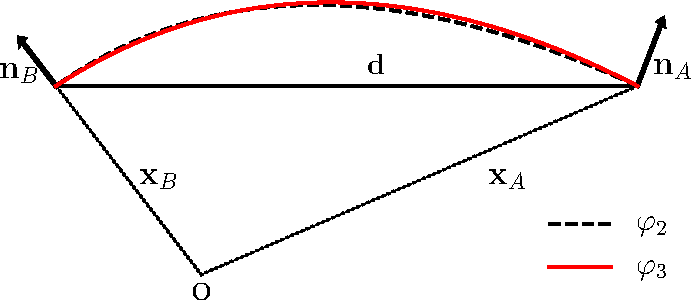
\includegraphics[width=0.8\linewidth]{fig/equivalence-crop}
\caption{Quadratic (dotted line) and cubic (red line) Nagata edge interpolants, for the case of well-behaved normal vectors.}
\label{fig:nagata}
\end{figure}
This process fails to give the expected results for a wide variety of pathological normal orientations. Singular points and their remedies have been discussed by Nagata.\cite{NAGATA2005327} For our purposes, it is sufficient that the interpolation will succeed for smooth surfaces, as is required by the ordinary Helfrich theory. It was discovered recently that the results for 
\begin{equation}
  \parens{\vec{n}_A \cdot \vec{d}}\parens{\vec{n}_B \cdot \vec{d}} \geq 0,
  \label{eq:nagfail}
\end{equation}
are problematic.\cite{NETO2013639}  Some of the issues are illustrated in Fig.~\ref{fig:recovery}. Namely, if both of the normal vectors are oriented in the same way with respect to $\vec{d}$, the quadratic interpolant will not lie in the angle between normal vectors viewed along $\vec{d}$. An example of this arrangement is given in the left panel of Fig.~\ref{fig:recovery}, where the two normals are approximately parallel and close to orthogonal to $\vec{d}$. Such a configuration of normal vectors may arise readily, e.g. from a normal estimation with a small perturbation of a flat mesh during the formation of a dimple. The resulting interpolant describes a large "sideways" bow, risking overlaps with other parts of the mesh. Similar problems occur in the event of twisting the normals as shown on the right of Fig.~\ref{fig:recovery}. If the interpolant were to lie within the space spanned by the normals and $\vec{d}$, it would have to contain an inflection point. 
For such cases, Nagata and subsequent authors advise either subdivide the mesh to cover the inflection point or to insert a flat line. In the case of a membrane simulation, such an approach is difficult to implement, as there are no underlying data to refine and a realistic expression of curvature is required. Furthermore, our experiments with updating the mesh with only quadratic patches were not successful. In order to ameliorate the situation, we increase the interpolation to cubic order:

\begin{figure}[b]
\centering
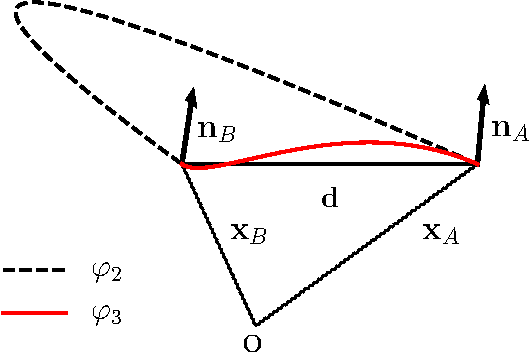
\includegraphics[width=0.49\linewidth]{fig/inflection_lcrop}
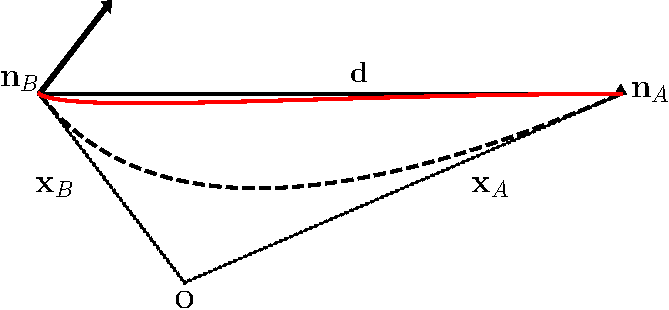
\includegraphics[width=0.49\linewidth]{fig/norf-crop}
\caption{Left panel: Quadratic (dotted line) and cubic (red line) Nagata edge interpolants, for the case of  normal vectors with equal orientation $\vec{n}_i \cdot \vec{d} > 0 $. Right panel: Arrangement for twisted normals with the additional condition of $\vec{n}_2 \cdot \vec{d} \approx 0 $.}
\label{fig:recovery}
\end{figure}

\begin{equation}
  \vec{\varphi}_3(t)
  =
  \vec{x}_A + \parens{\vec{d} - \vec{c}_1 - \vec{c}_2} t + \vec{c}_1 t^2 + \vec{c}_2 t^3.
\end{equation}
The derivative is given by
\begin{equation}
  \vec{t} = \vec{\varphi}_3'(t) = \vec{d} - \vec{c}_1 - \vec{c}_2 + 2 \vec{c}_1 t + 3 \vec{c}_2 t^2.
\end{equation}
% The tangent vectors at the endpoints now become
% \begin{subequations}
%   \begin{align}
%     \vec{t}_A \defeq \dd{\vec{\varphi}}{t}(0) &= \vec{d} - \vec{c}_1 - \vec{c}_2,
%     \\
%     \vec{t}_B \defeq \dd{\vec{\varphi}}{t}(1) &= \vec{d} + \vec{c}_1 + 2 \vec{c}_2.
%   \end{align}
% \end{subequations}
As before, we impose the requirement of the tangent vectors to be perpendicular to the normals at the endpoints. The introduction of $\vec{c}_2$ means that the equation system now has four degrees of freedom left to determine. Note that, e.g. the arc-length variation of a curve between two points, for a given set of tangent vectors will result in a straight line with an infinitesimal kink; it is therefore expected that an arbitrary increase of polynomial order will lead to an equivalent result. In order to achieve a good interpolant, it is necessary to require additional conditions. For the pseudoinverse operation to work, these conditions have to come in the form of linear equations.
Therefore, we impose an additional estimate of the binormal vector. This vector is orthogonal to the normal vector and is estimated to be normal to the plane spanned by $\vec{n}$ and $\vec{d}$, the construction is intended to keep $\vec{\varphi}_3'$ nearly parallel to $\vec{d}$. This leads to the following set of conditions:
\begin{subequations}
  \begin{align}
    \vec{n}_A \cdot \vec{t}_A &= 0,
    \\
    \vec{n}_B \cdot \vec{t}_B &= 0,
    \\
    \parens{\vec{d} \times \vec{n}_A} \cdot \vec{t}_A &= 0,
    \\
    \parens{\vec{d} \times \vec{n}_B} \cdot \vec{t}_B &= 0.
  \end{align}
\end{subequations}

As remarked previously, using the pseudoinverse for an underdetermined system corresponds to solving a least squares problem in the coefficient vector. This problem has an analytical solution, which we provide in the Supplementary Material, together with the detailed algorithm which produces the edge interpolant with a few vector multiplications.
We find them to be well-behaved, resulting in an interpolant very close to the original Nagata formulation for the ``nonpathological'' cases as well as a reasonable inflection point for the failure mode described in Eq.~\eqref{eq:nagfail}. The additional condition introduced minimizes the chance of edge overlap. 
%One can expect that there are going to be pathological cases for certain values of $a$, $b$, $c$, $d$, and $e$. Let us ignore this issue for the moment.
\subsubsection*{Interpolation of a Patch}
In order to create a surface interpolant, the edge interpolants have to be assembled into a surface. The patch interpolant $\vec{x}_2(\eta, \zeta)$ for the original quadratic Nagata edges is also of second order:
\begin{equation}
  \label{eq:interpolant}
  \vec{x}_2(\eta, \zeta)
  =
  \widetilde{\vec{c}_{00}}
  +
  \widetilde{\vec{c}_{10}} \eta
  +
  \widetilde{\vec{c}_{01}} \zeta
  +
  \widetilde{\vec{c}_{11}} \eta \zeta
  +
  \widetilde{\vec{c}_{20}} \eta^2
  +
  \widetilde{\vec{c}_{02}} \zeta^2.
\end{equation}
The six coefficients of this polynomial are determined by the requirement of the edges of the surface interpolant being equal to the edge interpolants. More precisely, the functions $\vec{x}_2(\eta, 0)$,  $\vec{x}_2(1, \zeta)$, $\vec{x}_2(\eta, \eta)$ have to be exactly equal to the Nagata edge interpolants. For a visualization of the structure, see Fig. \ref{fig:patch}. The edge polynomials restrict the domain of the interpolated patch to $0 \leq \eta \leq 1$ and $0 \leq \zeta \leq \eta $. 

\begin{figure}[hbt]
\centering
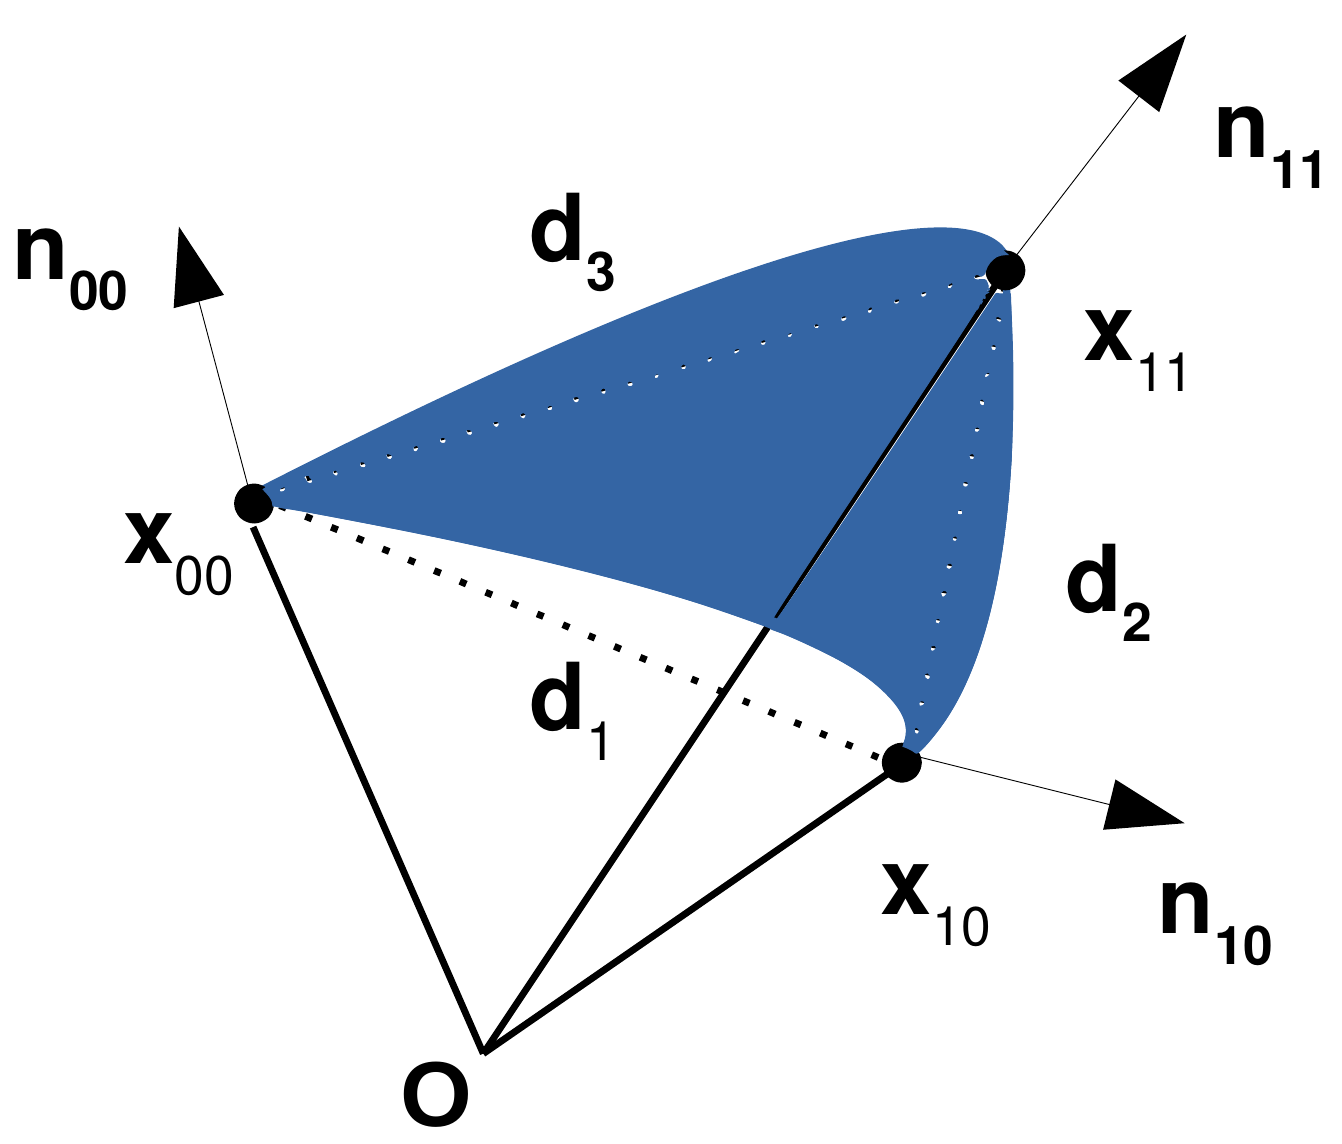
\includegraphics[width=0.5\linewidth]{fig/schema_f.png}
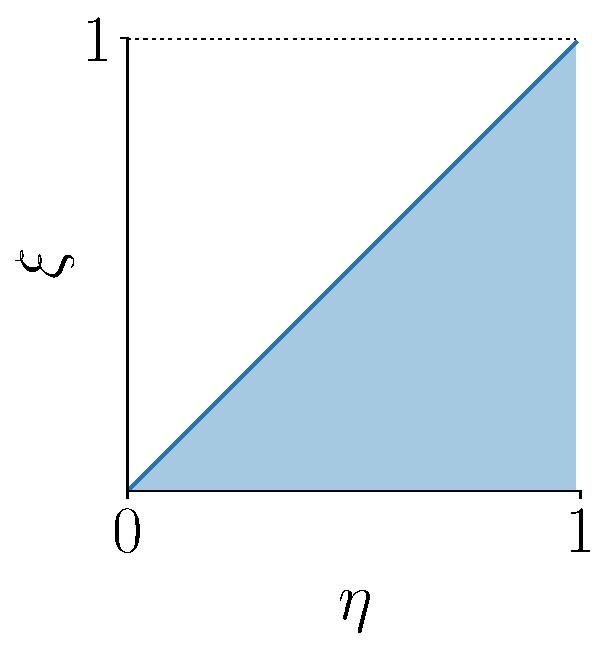
\includegraphics[width=0.39\linewidth]{fig/domain}
\caption{Left panel: Schematic of a patch interpolant as constructed from the edge interpolants. Right panel: Domain of the patch interpolant.}
\label{fig:patch}
\end{figure}

The third-order patch interpolant requires additional conditions to be uniquely determined. It must reprodcue the quadratic case when $\vec{c}_2 = 0$, resolving any ambiguity. A detailed derivation is given in the Supplementary Material. In our code, cubic edges are only used where the failure condition in Eq.~\eqref{eq:nagfail} is met as the alternatives of permitting bad interpolants or inserting a straight line lead to heavy artifacts. Excluding these configurations leads to the necessity of creating complicated, collective motions of the mesh (clustered moves) to avoid trapping. The stand-alone accuracy of the resulting interpolant is evaluated in the Results section.


\subsection*{Evaluation of the Helfrich Energy}
 For a closed surface, the Helfrich free energy $F$, supplemented by surface tension $\sigma$ and pressure $p$ terms can be stated as 
 \begin{equation}
  F = \int_\mathrm{Surf.} \D{A}  \bigg\{ \frac{{\kappa}}{2} (\tilde{H}-J_S)^2 + \bar{\kappa} K_G  + \sigma \bigg\} +\int_\mathrm{Vol.} \D{V} p.
  \label{eq:helf}
 \end{equation}
In this equation, the geometrical quantities include the total curvature $\tilde{H}$ (the sum of principal curvatures, in contrast to the standard definition of the mean curvature $H=\frac{1}{2}\tilde{H}$), the Gaussian curvature $K_G$, the area element $\D{A}$ and the volume element $\D{V}$. The material parameters are the bending rigidity $\kappa$, the Gaussian bending modulus $\bar{\kappa}$ and the spontaneous or intrinsic curvature $J_S$. The pressure $p$ and surface tension $\sigma$ can be interpreted as Lagrange multipliers on the total surface and volume, respectively. In our scheme, $A$ and $V$ are controlled instead by quadratic penalties and $K_G$ can typically be ignored due to the Gauss-Bonnet theorem. We note, that $V$ can be obtained from the divergence theorem using the spatial coordinate $\vec{r}$ as
\begin{equation}
 V = \frac{1}{3} \int_\mathrm{Vol.} \nabla \cdot {\vec{r}} \,\D{V} =  \frac{1}{3} \int_\mathrm{Surf.}   \vec{x} \cdot \hat{\vec{n}} \,\D{A},
\end{equation}
where $\hat{\vec{n}}$ is the surface unit normal vector as computed from the patch interpolant $\vec{x}$. If the surface is closed, it is sufficient to work with surface integrals to evaluate all of $F$. The surface integral is summed over all patches and in each patch is discretized on the domain of the interpolant using a seventh-order Gaussian quadrature scheme\cite{https://doi.org/10.1002/nme.1620120107}. Note the facility of constructing parallel planes accounting explicitly for separate monolayers and the availability of a reasonable direct way to evaluate Gaussian curvature on a face. 
If the surface is open, an additional term
\begin{equation}
    F_{\Gamma} = \int_{\partial \Gamma} \big[ \overline{\kappa}k_G + \tau \big] \mathrm{d} \mathbf{l}
\end{equation}
needs to be added, where the integration is performed along the boundary $\partial\Gamma$ of the surface, and a geodesic curvature $k_G$ as well as line tension $\tau$ of the membrane need to be integrated along the line element $\mathrm{d}\mathbf{l}$.
%\begin{equation}
% \Phi =  \int_0^1 d\eta \int_0^\eta d\zeta f(\eta,\zeta) \| \vec{x}_\eta(\eta,\zeta) \times \vec{x}_\zeta(\eta,\zeta)\| 
On the level of the code, different energy functionals are available via subclassing and all of the above described terms can be computed. Some further possibilities are described in the Supplementary Material, most notably an implementation of area difference elasticity (ADE)\cite{PhysRevA.44.1182,PhysRevE.49.5389} via control of the integrated mean curvature. Local curvatures can be expressed in a simplified manner by the coefficients. More details about the implementation are given in the Supplementary Material.

\subsection*{Parallelized MC Implementation}
\subsubsection*{Moves}

We use a standard Metropolis Monte-Carlo (MC) algorithm to evolve the interpolated surface and sample the Boltzmann distribution of the underlying energy functional. The advantage of this setup is that fluctuations, such as membrane undulations are automatically included in the simulation results. The sampling of a finite temperature distribution also implies our code is not an optimization code.
In contrast to standard DTS, we also have to consider the changes of the normals in the sampling of equilibrium geometries. We provide vertex moves, normal moves and so-called deep vertex moves. In addition to this, we have also implemented a basic bond-flipping ``Alexander'' move and a new type of move associated with lipid composition on a face. Due to the local nature of these moves, the code is easily parallelizable. In Fig.~\ref{fig:moves}, we show the part of the local mesh that is modified, as it needs to be checked for validity and is updated in every step. 
\begin{figure}[hbt]
\centering
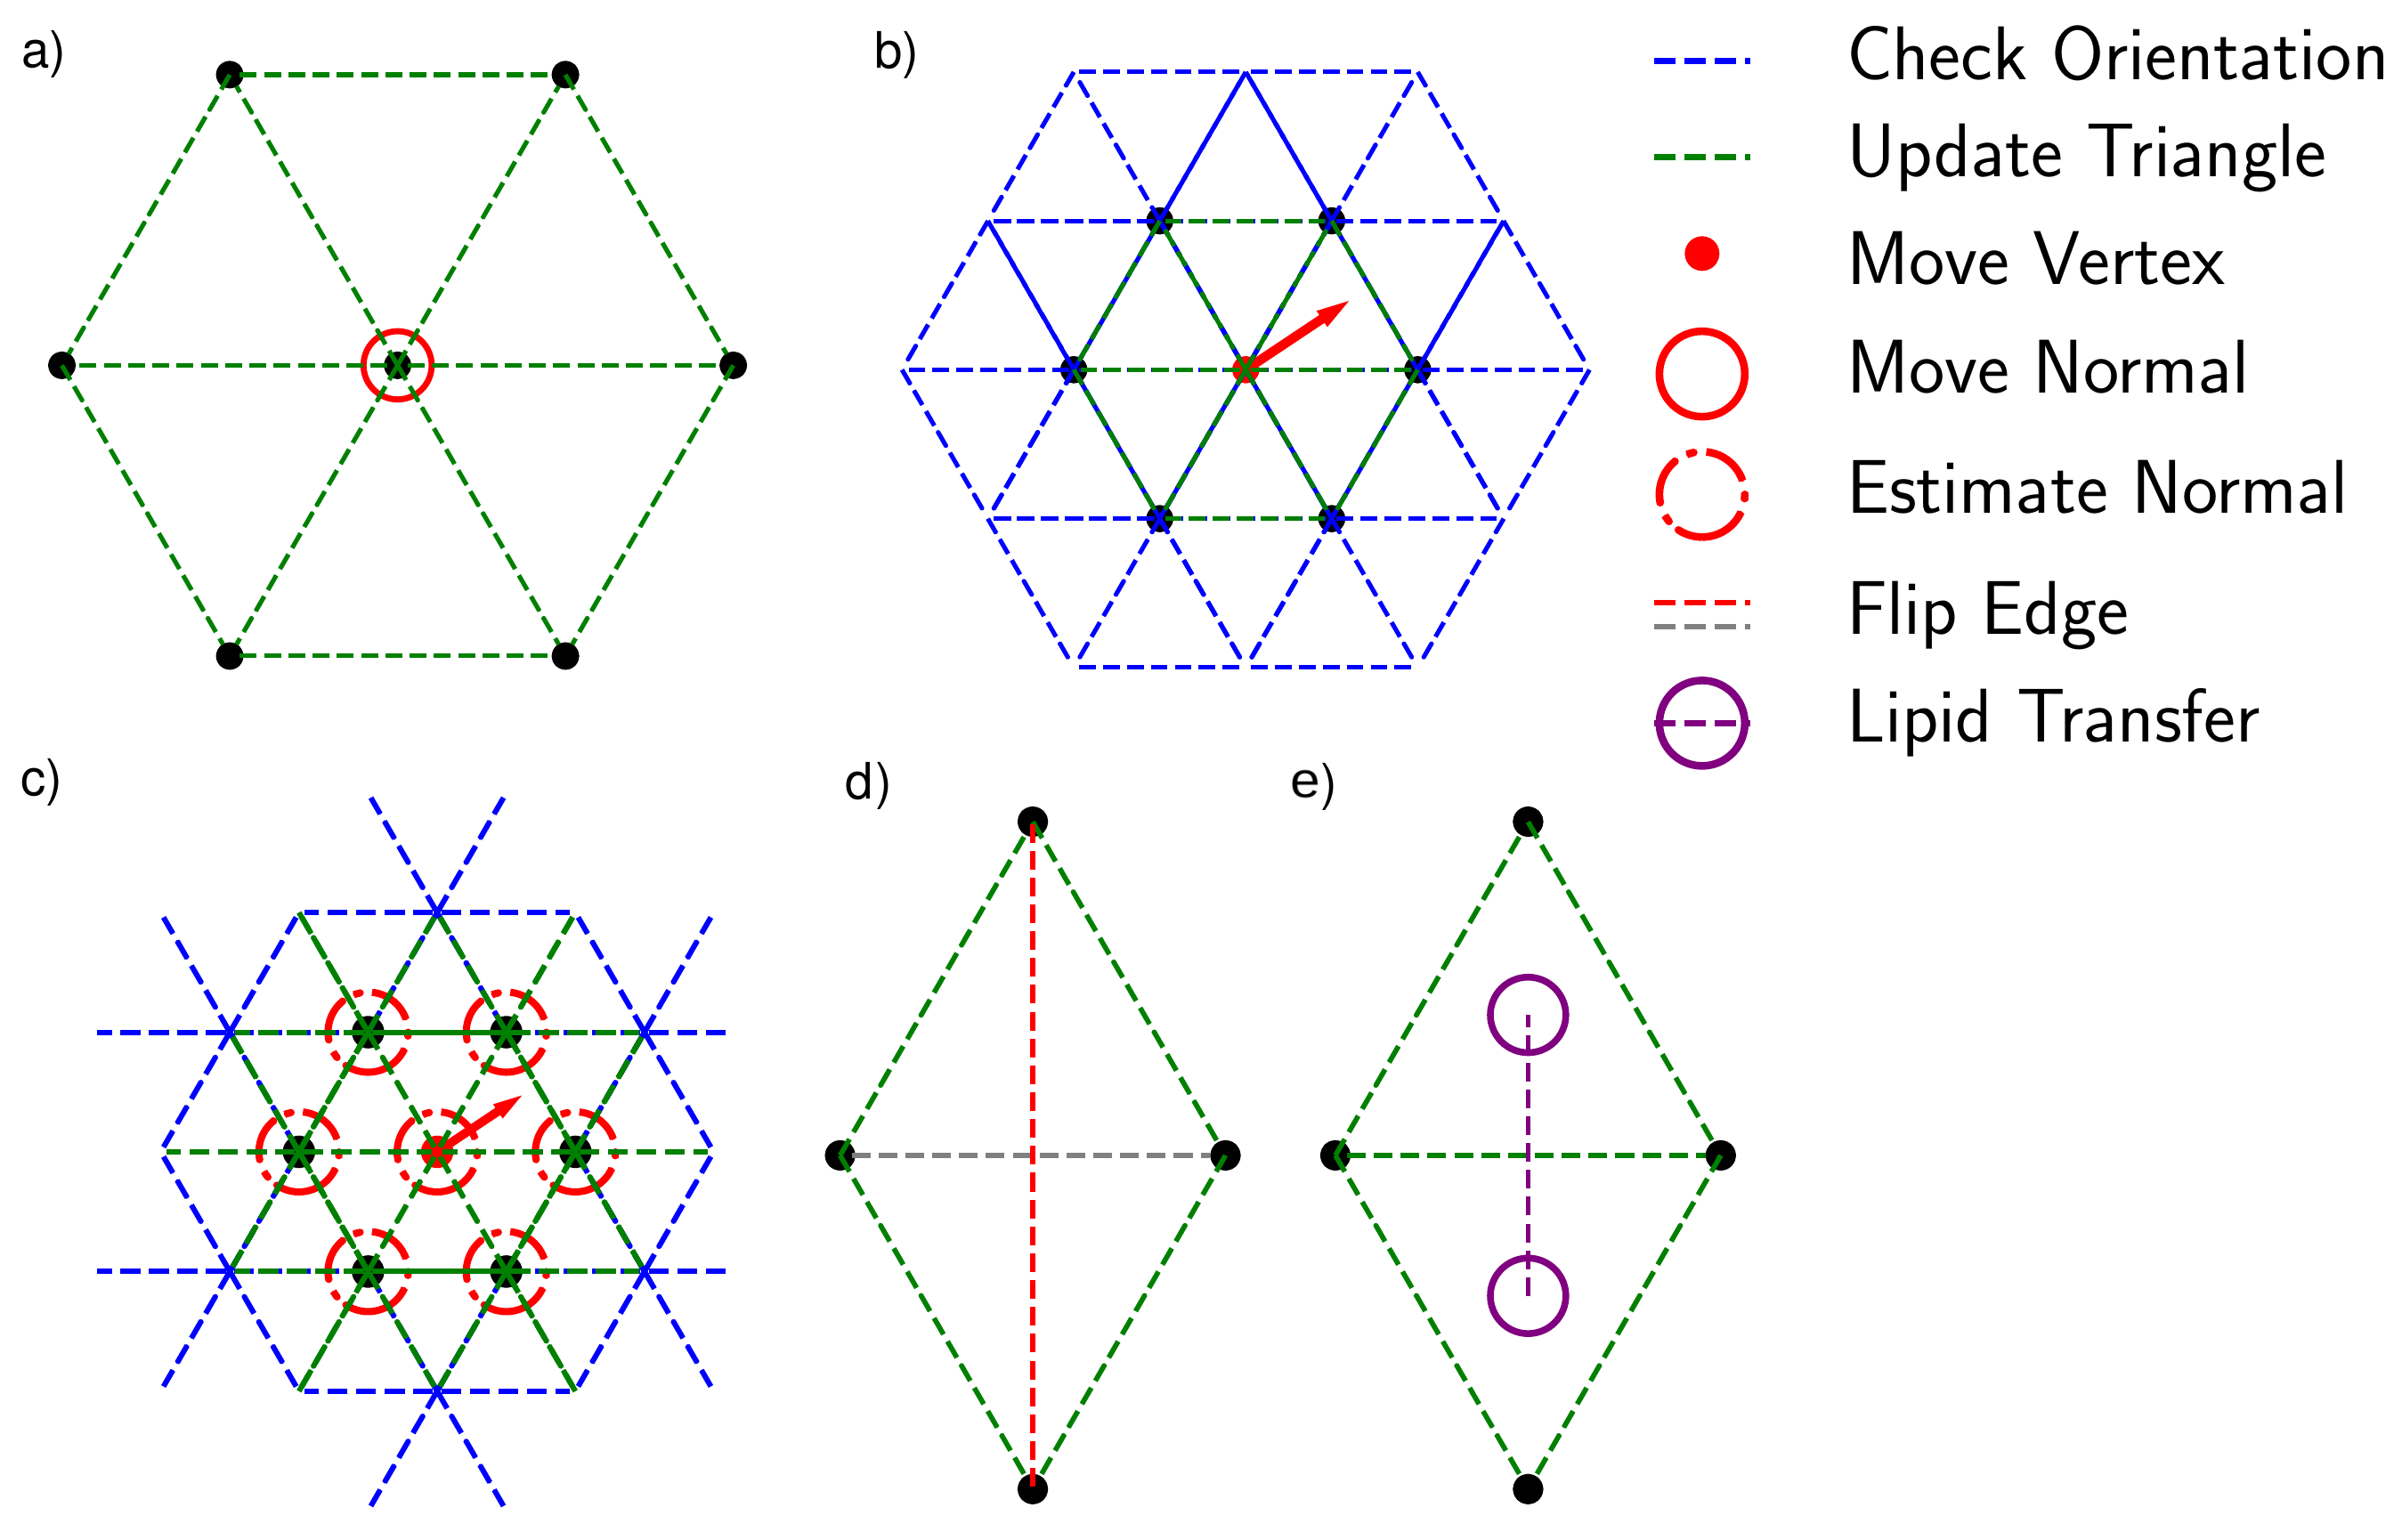
\includegraphics[width=\linewidth]{fig/moves.png}

\caption{Implemented MC-moves: a) Normal move and its update range, b) vertex move and it is update and face orientation check range, c) Deep vertex move, d) Alexander move, e) Lipid transfer move.  The legend describes the update schemes, face updates and orientation checks.}
\label{fig:moves}
\end{figure}
The \textbf{normal move} does not change any of the mesh vertices. In order to generate the move,
we create a vector $\vec{d}$ from a Gaussian distribution
\begin{equation}
   d_i = \zeta ; P(\zeta) = \frac{1}{\sigma \sqrt{2 \pi}} e^{\frac{-\zeta^2}{2\sigma^2}}, 
\end{equation}
where the components $d_i$ are set to separate Gaussian random variables. The pseudorandom variables $\zeta$ are generated using a Mersenne-Twister algorithm, initialized by a time-dependent seed. The proposed new normal vector is then obtained as 
\begin{equation}
 \vec{n}_P = \frac{\vec{n} + \vec{d}}{\| \vec{n} + \vec{d} \|}.  
\end{equation}
Note that the probability of proposing $-\vec{d}$ is the same as the probability of proposing $\vec{d}$, due to the symmetry of the Gaussian distribution. The variance, $\sigma$, can be adjusted automatically. For proposal probability, we find
\begin{equation}
\label{eq:reverse}
 P(\vec{n}_P  | \vec{n} )   = P(\vec{n}  | \vec{n}_P),  
\end{equation}
which helps to ensure detailed balance and allows us to compute the acceptance probability as
\begin{equation}
\label{eq:accept}
 A(\vec{n}_P | \vec{n} ) = \min \big\{ 1, e^{- \beta \Delta F} \big\}, 
\end{equation}
where $\Delta F$ is the change in the total free
energy
associated with the move and $\beta = (kT)^{-1}$. We state $F$ in units of $kT$, cancelling $\beta$. The change in energy can be computed locally by considering only the triangles which contain this normal, hence it is trivially parallelizable.
The only difficulty 
pertains to the evaluation of changes
to the global quantities $V$ and $A$.
For a global ``restraint'' on a function $\Phi$ to $\Phi_0$, with an energy contribution of the form 
\begin{equation}
 \frac{\lambda}{2}(\Phi-\Phi_0)^2 = F_\Phi. 
\end{equation}
The change $\Delta \Phi$ due to a local MC step leads to an energy change of
\begin{equation}
  \Delta F_\Phi = \frac{\lambda}{2}\Delta \Phi(\Delta \Phi-2(\Phi-\Phi_0)). 
  \label{eq:global}
\end{equation}
This means, that a local scheme requires the storage of the current global value $\Phi$. However, $\Phi$ can be updated  using $\Delta \Phi$ if the current local contribution to $\Phi$ is stored on the face. In order to accept the proposed normal, it will also have to produce valid cubic or quadratic face interpolants.
To ensure this, we require the proposed normal to be at a minimum angle to the other triangle normals $\vec{n}_i$, so that
\begin{equation}
 \vec{n}_p \cdot \vec{n}_i > \epsilon = 0.01.  
\end{equation}
Finally, a collision check is performed. This collision check is delayed because of the great computation expense of evaluating the neighbor list. 
The second move to consider is the \textbf{vertex move}. Again, a vector is sampled from a normal distribution and added to the previous position.
The same sort of symmetry argument, leading to Eq.~\eqref{eq:reverse} applies. The change of a vertex has more spatially extended consequences than the change of a normal, see Fig. \ref{fig:moves}, b). Of course, the triangles in the immediate vicinity of the initial vertex have to be updated. The acceptance criterion in Eq.~\eqref{eq:accept} is applied.
Moreover, the acceptance of the vertex move requires \begin{equation}
 \sphericalangle(\vec{x}_i,\vec{x}_j,\vec{x}_k) > \frac{\pi}{16},
\end{equation}
for all of the angles in the triangle. 
The ``\textbf{deep-vertex}'' move from Fig.~\ref{fig:moves}c, removes the normal vectors as independent degrees of freedom, determining them by the faces of the underlying triangular mesh. The way this is achieved is by reconstructing all normals affected by a vertex move, i.e. all normals on vertices neighboring the modified vertex are re-estimated using our normal estimation algorithm.
Under these conditions, the move is fully reversible. This would not necessarily be true if the move was to only update the normal on its own vertex, because under these conditions the vertex normals of the surrounding faces would no longer correspond to their estimated values. As a remedy, we ``quench'' the normals to their estimated values before using this move or to use it standalone. Because of the potential issues, this move has been deactivated by default. Our MC scheme is also set-up in such a way as to minimize irreversibility by the organization
of the Markov chain. In particular, for each degree of freedom, multiple trials\cite{4f63006b-689a-3636-a6e6-a36d119d0657} are  proposed until acceptance, so that for each MC step (almost) all degrees of freedom have moved. The total step can, therefore, be interpreted as a factorization of individual symmetric steps.\cite{10.3389/fphy.2021.663457} Furthermore, we have implemented a mechanism of automated propagation, which ensures all other energy carrying objects are updated together with the faces, such object can e.g. include edge terms. Algorithmic details on the MC scheme and the automatic construction of decoupled parallel execution loads are given in the Supplementary Material.
The \textbf{"Alexander"/bond-flip move} show in Fig.~\ref{fig:moves}~d) is currently set to be accepted only if it decreases energy. Our automatic parallelization  scheme, described in the SI relies on tracking
 the dependencies of each degree of freedom as determined from mesh. As the move changes the mesh topology, the parallelization structure of the code needs to be updated, and neighbor lists rebuilt after each round of bond-flipping moves. Hence, the remeshing move is executed only occasionally and (mostly) serially. As the number of faces is conserved, face properties (such as local bending rigidity) can remain associated with a fixed face, currently, no redistribution occurs. The Alexander move is associated with the edge which is flipped. The \textbf{lipid mixing} move shown in Fig.~\ref{fig:moves}~e) is also edge-associated, random lipids are chosen from the population of both faces and transferred to another face. More information is found in the lipid mixing section.

\subsection*{Mesh Properties and Constraints}

\subsubsection*{Constraints}

It is possible to selectively block or remove parts of the mesh from active evolution. The former can be accomplished by removing some properties while retaining the mesh points. The latter is accomplished via \textit{block} objects, which prevent updating parts of the mesh, e.g. only the $x$ coordinate of a vertex or a normal. Blocks provide a simple way of implementing sophisticated boundary conditions. As an example, it is possible to allow the boundary of the mesh to evolve in-plane only while the normal vectors, and hence the tangent basis is kept constant. The block objects can also be used to suppress remeshing and lipid flow across membrane edges. We provide a utility to load simple coordinate and normal freezes via text files. The final distribution of our software contains a manual and selection tools to assist with preparing the blocks. By editing the source code, block objects can also be used to constrain curvilinear coordinates.



\subsubsection*{Face Properties}
As energy and integral evaluations are performed over the faces, it makes sense to also store information about the parameters $\kappa, J_s, A_0$ and others on them. In fact, each face contains an arbitrary collection of properties, which are accessed via a text key. Such properties can be assigned at load as well as at run time and are automatically included in output visualizations. This allows us to dynamically store and export information about composition as well as to compute modified elastic properties and local coupling terms on the fly. 

\subsection*{Lipid Mixing}

The implemented energy functionals would also allow to compute the energy directly for a composition. However, a proper implementation of lipid mixing requires the lipid composition to be dynamic and, therefore, requires the definition of mixing rules and moves which manipulate it. Ideally, the modification of the lipid composition should be transparent to most of the energies computed from it. In the literature,
it has often been proposed to compute the bending rigidity $\kappa$ as\cite{doi:10.1021/ct400492e,doi:10.1021/la00047a035} via a harmonic average of the single lipid moduli $\kappa_i$:
\begin{equation}
 \frac{1}{\kappa} = \sum_i \phi_i \frac{1}{\kappa_i}.
\end{equation}
Here $\phi_i$ refers to the volume fraction, which is calculated as 
\begin{equation}
 \phi_i = \frac{m_i A_i}{\sum_j m_j A_j}, 
\end{equation}
with $A_i$ the area per lipid of the lipid species $i$. This means, that we assume that the area per lipid does not change while mixing. The area per lipid $A_i$ is a reference area contributing to $A_0$, so that mixing/bending and stretching are not coupled. By $m_i$, we refer to the number of lipids of species $i$ present in a triangle.
Of course, completely different behavior is possible.
An example occurs during a phase transition to gel or L$_O$ phase. As long as the behavior is well-defined it is easy to implement the requisite models in our code.
The spontaneous curvature is computed as
\begin{equation}
 J_s = \sum_i \phi_i c^0_{s,i},
\end{equation}
where $c^0_{i}$ is spontaneous curvature of the pure $i$.\cite{Andelman_1994, Khelashvili20091626}
We have recently tested the validity of these equations against atomistic molecular dynamics results.\cite{Konar2023.02.06.527315}
Furthermore, the mixing entropy of the lipid composition with a total occupancy of lipids $M$ on a side/leaflet of a triangle can be estimated as ideal in the surface fractions\cite{Andelman_1994}:
\begin{equation}
 F_\mathrm{mix} = kT M \sum_i {\phi_i} \mathrm{ln} \phi_i. 
\end{equation}
This free energy is added to the energy in the form of a penalty. In this way, it can be used with all energy functionals. Real valued molar fractions $\phi_i$ and lipid occupancies $m_i$ presume that the lipid composition of a triangle is a macroscopic quantity. As the mixing entropy is temperature dependent, the temperature is provided via the inverse temperature $\beta$. 
Furthermore, both leaflets in a bilayer are considered, and their properties are computed separately, and then added together. The curvature $c_0$ is added with an inverse sign to that of the opposite leaflet.
The equilibrium area of a face $A_0$ is computed from the areas per lipid on each leaflet, the $A_0$ are then averaged (we recommend setting up the simulation with equal $A_0$ for both leaflets).
The implemented approach models only the bilayer midplane, so that the finite and variable thickness of the actual bilayer is neglected. 
There is also the possibility to use a stylized protein, whose move will be integer valued and which will override the curvature generated by the lipids.
In order to simulate lipid mixing, an exchange move has been implemented. On each leaflet:
\begin{enumerate}
 \item Select two lipid types at random from adjacent faces.
 \item Generate two random amounts of lipids to be moved.
 \item Move the two lipids between the adjacent faces and recompute the energies, including mixing energy.
 \item Accept or reject the move.
\end{enumerate}
 Uniform random numbers are used for the exchange move. In order for the move to be allowed, the total occupancy must be above a certain threshold, e.g. zero. Currently, the moves are set so that the total $A_0$ of each face and leaflet does not change by lipid exchange flow. This serves to prevent mesh degeneration. While we are not aware of an equivalent implementation, similar ideas have been explored in the past.\cite{Kumar2001}

\subsection*{Collision Detection}

In a naive implementation, the detection of potential collisions between any pair of elements in a set of $n$ triangles requires $\mathcal{O}(n^2)$ operations. To mitigate the computational expense of the collision detection, we implemented a neighbor-list based \textit{broad} \cite{ericson2004real} search that aims to reduce the number of explicit intersections which have to be computed. The broad search is followed by a \textit{narrow} phase that relies on the popular \cite{kurniawan2019surface, landstorfer2021mesh, mandal2022interactive} fast triangle-triangle intersection test of Möller \cite{moller1997fast}. As the mesh faces are cubic surfaces, the use of the Möller algorithm is a compromise between precision and computational cost.


\subsection*{Penalties and Errors}
For the calculation of the energy, and the consistency of the interpolation, we require a consistent definition of the surface integral everywhere on the surface and to evaluate the same for an arbitrary subdomain
\begin{equation}
  \int_\mathrm{Patch} f \, \mathrm{d}A, 
\end{equation}
where $f$ may depend on derivatives of the surface or might be a differential form.
For example, a smooth surface in $\mathbb{R}^3$ will fulfill
\begin{equation}
 \int_A  \nabla \times \hat{\vec{n}}  \cdot \mathrm{d}\vec{A} = \oint_{\partial A}  \hat{\vec{n}} \cdot \mathrm{d} \vec{l} = 0,
\end{equation}
%and \cite{doi:10.1137/1027143}
%\begin{equation}
% \int  H  \hat{\vec{n}}  \mathrm{d}A = %\oint_{\partial A}  \hat{\vec{n}} %\times %\mathrm{d} \vec{l} = 0   
%\end{equation}
for any closed, finite area $A$ with boundary $\partial A$, tangent vector $\mathrm{d}\vec{l}$ and oriented surface element $\mathrm{d}\vec{A}$, and . It is easily shown that $\nabla \times \hat{\vec{n}} = 0 $ is fulfilled everywhere inside an interpolated patch. If $\mathrm{d}\vec{l}$ is a tangent vector of an edge interpolant, integrating around the boundary of each patch will also fulfill the condition as even where normals are ambiguous/discontinuous on the edge interpolant, both are orthogonal to the tangent vector which follows the boundary line by construction. 
However, we need more regularity than this, as we are interested in integrals of $\tilde{H}$ and $\tilde{H}^2$. On a patch boundary, one of the tangent vectors, i.e. the one taken along the edge interpolant is identical to that of its neighboring patch. Away from the vertex, the other tangent vector may be different so that for an identical point at the edge two different tangent vectors are obtained. \textit{Quasi}-tangent continuity means that tangent continuity is ensured only at the vertices so that
in general, our interpolant is only $\mathcal{C}^0$ continuous, across edges but the computation of curvature requires derivatives of $\vec{n}$ in any direction, in particular the total curvature $\tilde{H}$, i.e. the covariant normal divergence
\begin{equation}
  \tilde{H}  = \nabla \cdot \hat{\vec{n}},
\end{equation}
has to be (square) integrable on the surface. At the edge, one  tangent vector is shared (hence the same normal curvature in one direction\cite{do2016differential}). If the normal vector at this point is also identical, it is possible to construct a local orthogonal tangent basis, this second tangent ($  \vec{t}_\bot$) defines a shared normal $\hat{\vec{n}}$ as it stands orthogonal to the edge direction and $\vec{n}$ at all times.
Tangent, i.e. $\mathcal{C}^1$ continuity is sufficient to guarantee some curvature integral properties, but does not guarantee continuity of the curvature itself.
Furthermore, numerical experiments showed that the patch interpolant does not always reproduce the vertex normals used to create it. For example, one of the edge interpolants may have parallel tangents at the endpoints during construction or might generate normal vectors of opposite orientation. Hence, before accepting a move it is verified that
\begin{equation}
 \hat{\vec{n}}_\mathrm{Mesh} \hat{\vec{n}}_\mathrm{Nagata} \geq 1-\epsilon.
\end{equation}
We use $\epsilon = 0.005$ as numerical tolerance for normal reproduction. In Fig. 4 of the Supplementary Material,  we show how enforcing normal reproduction helps to enhance tangent continuity. 
In order to bring the discretization closer to a $\mathcal{C}^1$ continuity, we define the following energy scale
\begin{equation}
 I = [(\kappa+1)(1+A_0J_s^2)+A_0^2K_A].
\end{equation}
The individual terms in this intensity are spatial-scale free energy units. They are set to cover all sources of energy in the problem so that a significant $J_s$ does not damage the regularizing penalty. 
Now, we split the tangent basis into two parts,
\begin{equation}
 \vec{t}_{=} = \vec{\varphi}' ; \vec{t}_\bot = \vec{\varphi}' \times \hat{\vec{n}}.  
\end{equation}
We then require that at the midpoint of an edge
\begin{equation}
 \hat{\vec{t}}_{\bot,m} \stackrel{!}{=} \frac{1}{2} (\hat{\vec{t}}_{\bot,0} + \hat{\vec{t}}_{\bot,1}),
 \label{eq:npenal}
\end{equation}
where the subscripts (0,1) denote the normalized average value of $\vec{t}_\bot$ at the endpoints of the edge interpolants. By controlling the evolution of $\hat{\vec{t}}_{\bot}$, in each triangle,
we enforce the continuity of normals at the center of the triangle, biasing towards $\mathcal{C}^1$ continuity without requiring information from adjacent triangles. Deviation from Eq.~\ref{eq:npenal} carries a quadratic penalty depending on $I$. In the Supplementary Material, we quantify the approximate tangent continuity and show its conservation in a production run.
We also penalize too small triangle areas (starting $<40 \% A_0$) and deviations from an equilibrium angle ($|\alpha| < 0.316$) with quadratic penalties proportional to $I$. The interpolant is highly tolerant of different penalties, as long as they are sufficiently strong. The area penalty serves mainly to prevent mesh degeneration. This mesh degeneration is less of a problem for the interpolant than for the MC algorithm, as the admissible step size becomes highly in-homogeneous. Similarly, the angle penalty mostly serves to prevent the locking and overlap of triangles. The numerical values of the penalty terms are given in the Supplementary Material.

\subsection*{Input and Output Formats}

The mesh input file format for this code is wavefront \textsc{obj}. Meshes of this format can be generated and exported from many free and standard tools. If the original obj file does not contain normals, they will be reconstructed from neighboring face normals in a simple weighting scheme\cite{Max1}.
The program also exports this type of mesh, in addition to \textsc{XML}-\textsc{VTK}\cite{vtkpara} unstructured grid files (.vtu). These are readily available and can be visualized and processed with the Paraview software package\cite{paraview}. 

\section*{Results and Discussion}
\subsection*{Example Meshes}

It is difficult to unit-test the error of the interpolation. The easiest way to proceed is to demonstrate the accuracy for example meshes. These example meshes are not the result of a simulation, but are generated geometric objects. The results are shown in Fig.~\ref{fig:unittests}. For the unit icosphere mesh Fig.~\ref{fig:unittests}~a), the corresponding values are a total curvature of 12.518, energy of 24.959$\kappa$ and area of 12.5662. The Gaussian curvature integral evaluates to 12.4707. The theoretical values for area, curvature and Gaussian curvature are $4\pi$ $\approx 12.5664$ for $R=1$. The theoretical energy is $8\pi \kappa$. The volume error is negligible. We also tested the icosphere using purely cubic interpolants. Area and volume accuracy remained unaffected, but energy decreased to 24.736$\kappa$ and curvature to 12.44. For the catenoid the absolute error was similarly increased by 0.24$\kappa$. We note, that the quadratic interpolation appears more robust, but errors remain small. At present, we do not know how important integration order is for error control. We fall back on the quadratic interpolant, when normals allow it. The toroidal mesh Fig.~\ref{fig:unittests}~b) has a total $K$ integral of -0.2 over the surface, the theoretical value is zero.
The catenoid mesh Fig.~\ref{fig:unittests}~c), mainly due to the difficult normal estimation at the edges, results in a total curvature integral of -0.27 over all faces and a total Helfrich energy of 0.22$\kappa$ over an area of 17.63 units. Any minimal surface has $H=0$ everywhere, so the theoretical value for mean curvature integrals is zero. The catenoid also has an Euler characteristic of 0. As such, integrating $K$ over the mesh and $k_G$ over the edges results in two terms canceling to 0.032, close to the expected result.. This illustrates the high accuracy of our scheme for good quality meshes. The flat triangle mesh Fig.~\ref{fig:unittests}~d) does have a mean and Gaussian curvature identically zero. Its $k_G$ boundary integral evaluates to 6.28, close to the theoretical value of 2$\pi$ for the Euler index of one. In the lower panel, we show the convergence of Gaussian and mean curvature for the platonic solids. For their computation, we used analytical normals.

\begin{figure}[hbt]
\centering
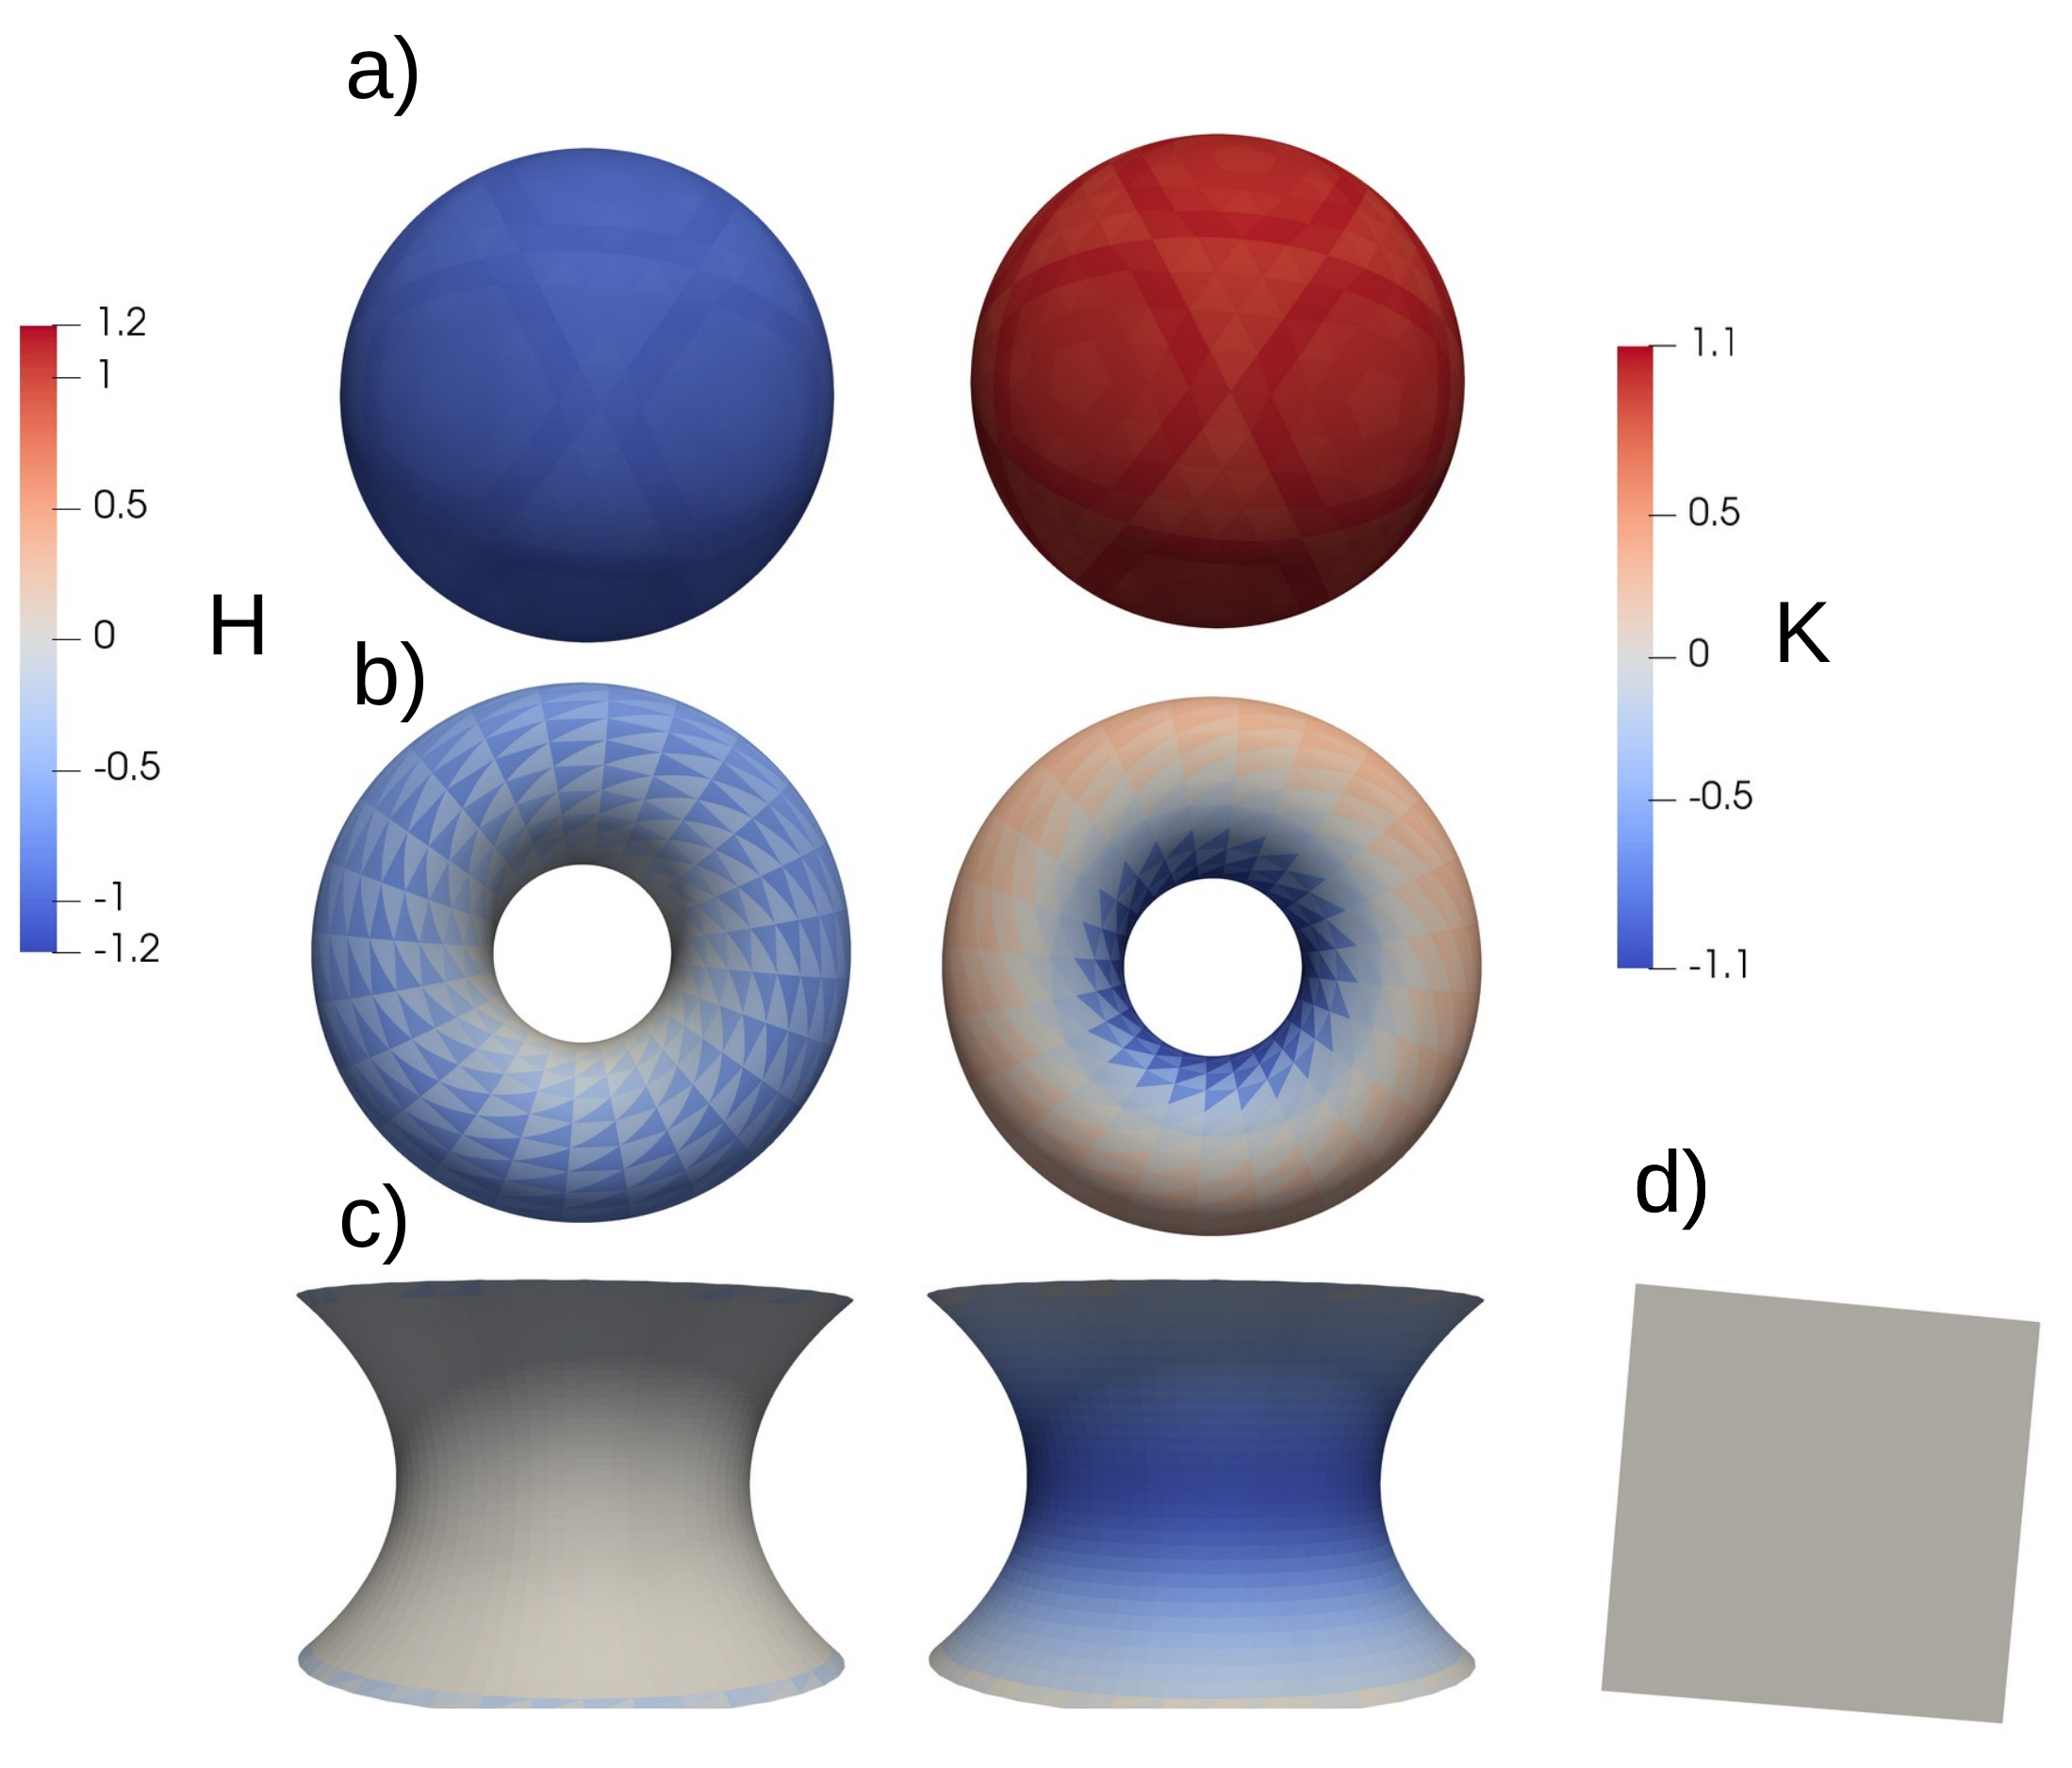
\includegraphics[width=0.8\linewidth]{fig/upper_new.png} \\
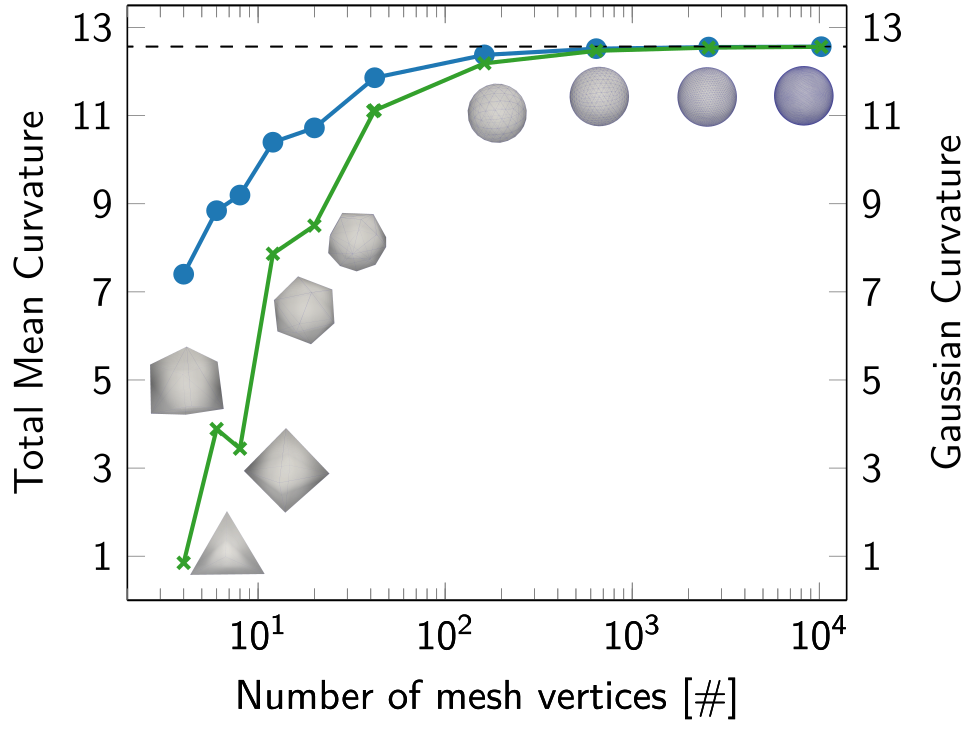
\includegraphics[width=0.7\linewidth]{fig/mergedkh.png} 
%\includegrapscanninghics[width=0.4\linewidth]{fig/norf}
\caption{Upper part: Four example meshes, with mean curvatures (left column) and Gaussian curvatures (right column) plotted as averages over face integrals, normal orientation gives negative H to the sphere. a) Icosphere mesh (642 vertices, 1280 faces) b) Toroidal mesh (1152 faces, 576 vertices), R$_1$=1, R$_2$ = 2. c) Catenoid Mesh. (2340 faces, 1209 vertices) Flat mesh (162 faces, 100 vertices. The mean curvature and Gaussian curvature scale are shared between meshes. Lower part: Convergence test of mean (blue) and Gaussian curvature (green) integrals for a range of platonic solids and icospheres.}
\label{fig:unittests}
\end{figure}



\subsection*{Helfrich Shapes}
In order to validate the interpolant and our MC algorithms, we reproduced the behavior of the known rotationally symmetric shapes of the Helfrich Hamiltonian. The corresponding minima have been well explored and confirmed recently by independent techniques.\cite{BIAN2020112758,cjmsolver} Results are shown in Fig. \ref{fig:diagram}. We have generated all the points using a discocyte starting geometry, by moving the volume restraint and keeping the area constant. In particular, thanks to the MC implementation we are able to transform prolate to discocyte and vice-versa near the theoretical limits, which are indicated by the dotted vertical lines with the numerical values marked in Fig \ref{fig:diagram}.\cite{BIAN2020112758,cjmsolver} The prolate state can be somewhat metastable, so that, with fast pulling some ``wormlike'' shapes were obtained. Discoid geometries readily transition to prolate ones: the point to on right of the line at $v_0$ 0.65 has a prolate long axis. The transition from discocyte to stomatocyte was also observed and occurred via collision and repulsion of the stomatocyte dimples. We provide documentation of these transitions as videos, showing how we can generate each shape from each other. The values we show for $v_0>0.1$, represent sampling averages over 20K steps, after more than 1M equilibration steps at the stationary shape as we have not implemented gradients. In theory, the minimal energy is $8\pi\kappa$ for the sphere at $v_0 = 1$, and $16\pi\kappa$ for the stomatocyte (in the limit a sphere inside as sphere), with a supralinear increase in the prolate regime.\cite{PhysRevA.44.1182}
The theoretical curve is shifted by the thermal energy $\alpha$. The value of $\alpha$ was estimated by comparing the minimal curvature energy of an icosphere at $v_0 = 1$ at rest, found when annealing only the normals and edge flipping at $\beta=1000$ to its simulation average energy at the simulation conditions, the difference is $\approx$ 0.7$\cdot 8\pi\kappa$. The geometries shown in Fig. \ref{fig:diagram} also show of the curvature on each individual face (only the average values are mapped on each face). 

\begin{figure}[hbt]
\centering
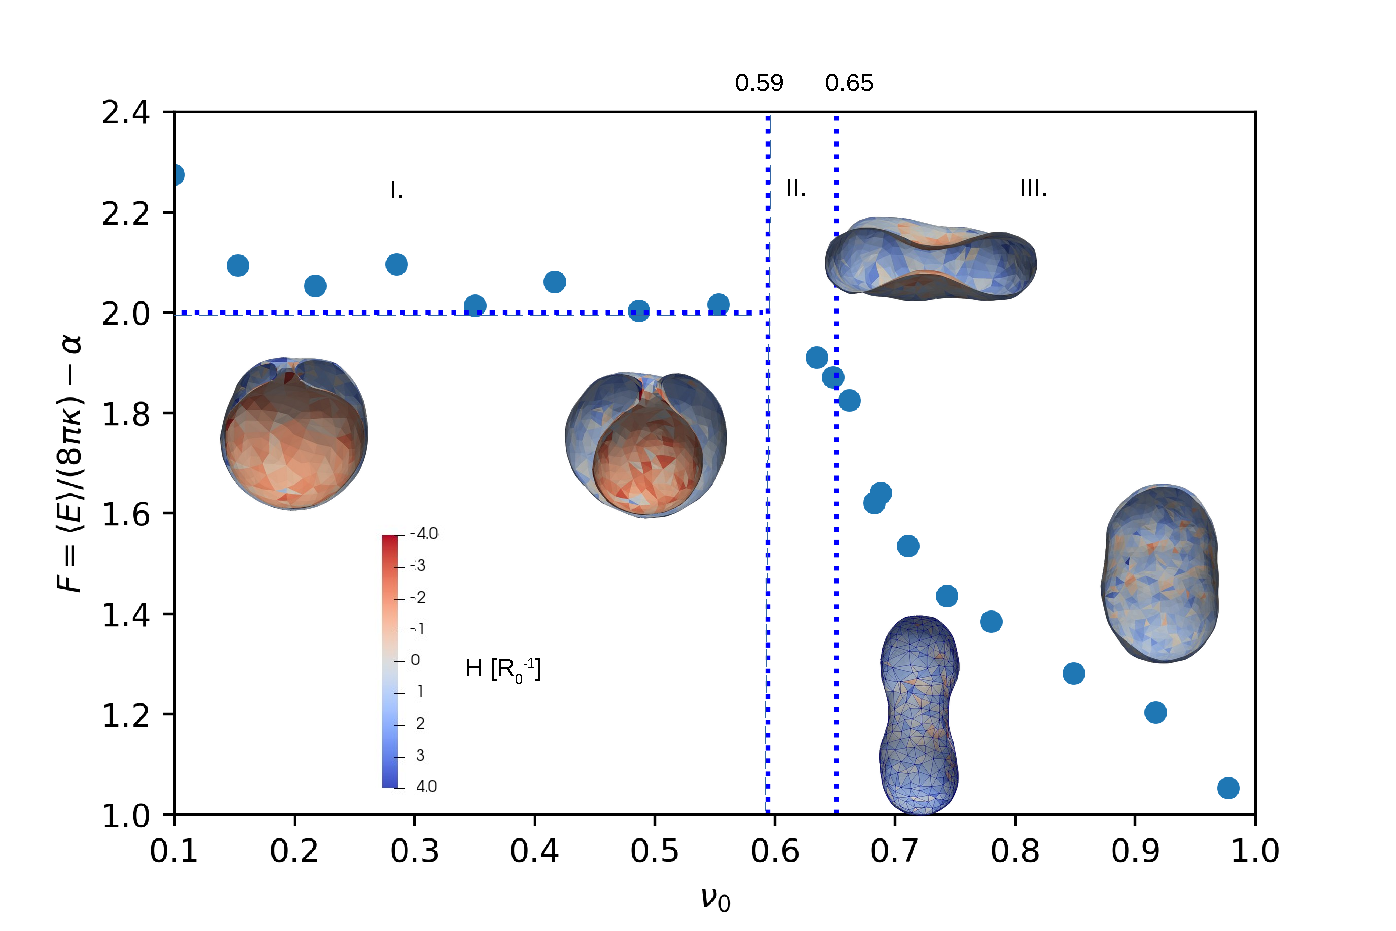
\includegraphics[width=\linewidth]{fig/Fig_phase_upd3-crop.pdf}
%\includegraphics[width=0.4\linewidth]{fig/norf}
\caption{Results for spherical vesicles, including the shapes for stomatocytes I., discocytes and oblate II., prolate  III. shapes obtained using volume and area constraints. The blue line indicates the theoretical value for the stomatocyte. $\alpha$ is due to the thermal energy of the degrees of freedom of the mesh. All results are derived from the 1280 face / 642 icosphere mesh. Starting point was a discocyte geometry. The energies are average values over the equilibrated part of the run.}
\label{fig:diagram}
\end{figure}


For this simulation, only the global surface area $A$ and the global volume $V$ were restrained. From these was computed the reduced volume
\begin{equation}
 \nu_0 = \frac{6V}{A^{3/2}}\sqrt{\pi}.
\end{equation}
When the space inside the vesicle becomes too small, i.e. at $\nu_0<0.2$ fluctuations deform the mesh and the neck becomes heavily penalized. While we believe it might be possible to go even lower with appropriate penalties, this seems to be quite sufficient for most stomatocyte shapes. In the Supporting Material we provide further simulation details. Equivalent inputs are also part of the OrganL distribution.

\subsection*{Examples: Curvature Bias and Lipid Mixing}

The sampling of the standard Helfrich minima in Fig.~\ref{fig:diagram} is just a precondition for the more advanced methods. With a robust description of the surface, it also becomes possible to add the lipid moves described in the previous section. For the purposes of clarity, we have chosen only one leaflet to have a strong curvature. In Fig. \ref{fig:examples} a), the comparison of a mixed patch with $J_s = 0$ is shown. A protrusion is stabilized by curvature-driven lipid demixing. 
The lipid population and local $J_s$ are visualized together in central and right panels. The boundary of the simulation is constrained. The lipid demixing effects in the example are intended for illustration purposes,
they result from the boundary conditions, lipid parameters and restraints applied, and do not indicate that ideal mixtures will spontaneously demix to create
deformations under realistic conditions.

\begin{figure}[hbt]
\centering
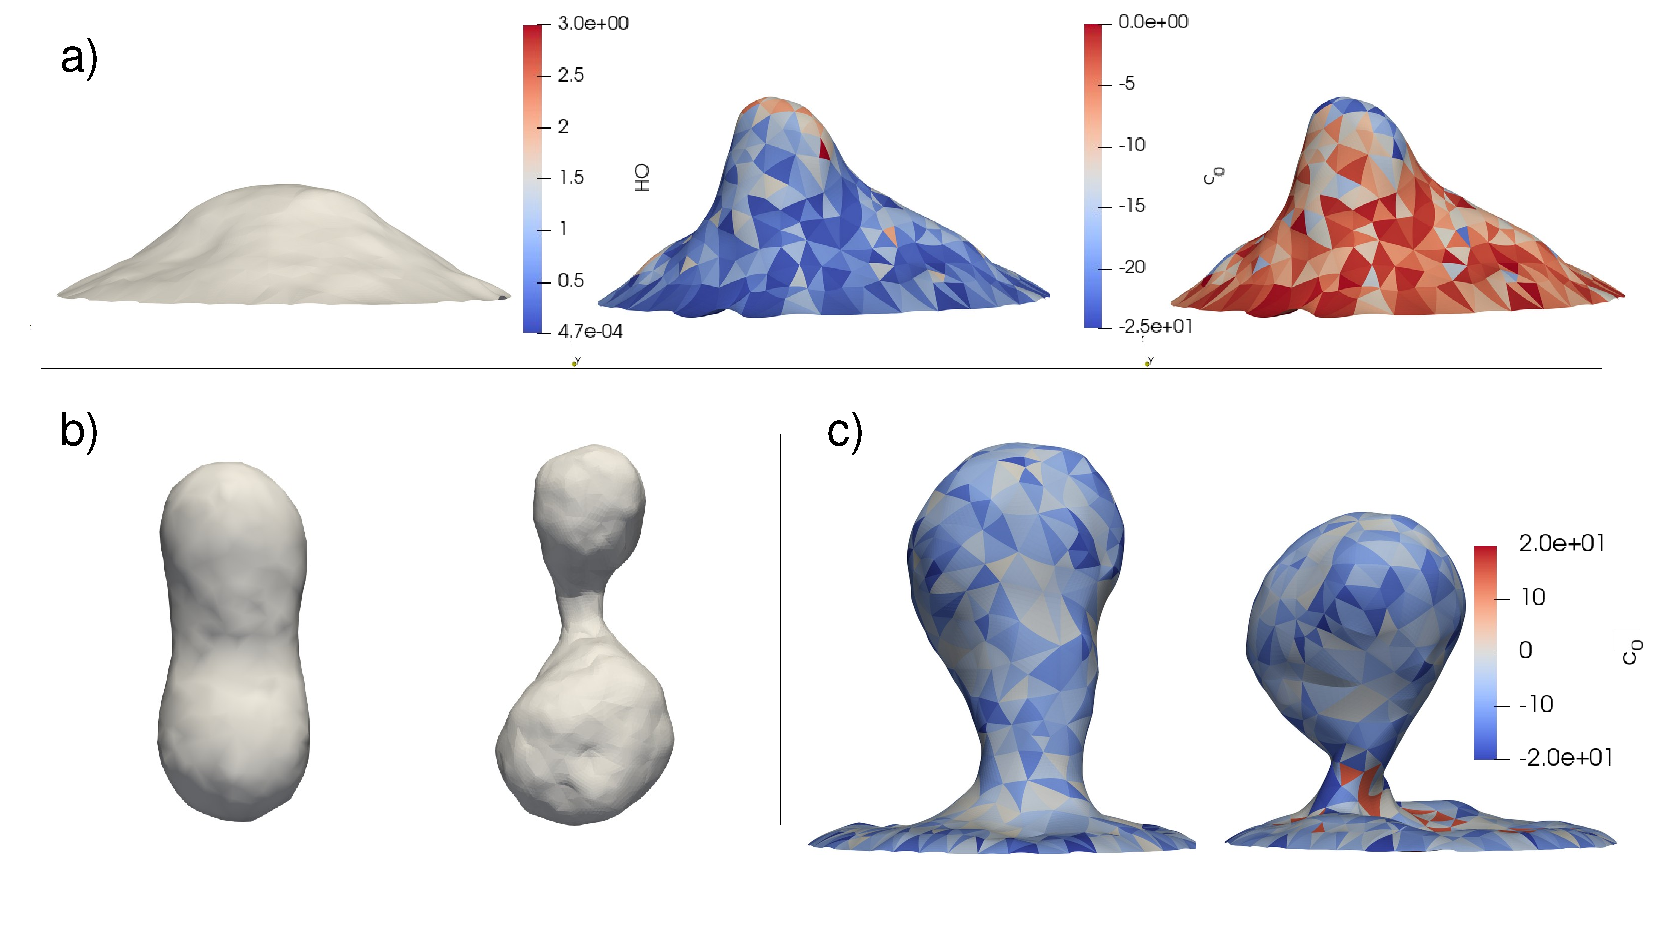
\includegraphics[width=\linewidth]{fig/Fig_exmp_upd2}
\caption{a) Coupling of lipid mixing and curvature generation with membrane geometry. Left panel: Simulation of lipid mixing without curvature, Central panel distribution of curved lipid and budding triggered by the same. Right panel, spontaneous curvature. b) ADE simulation starting from prolate geometry (left), as implemented by a global curvature restraint. c) Comparison of lipid budding and constriction with high spontaneous curvature (left), and neck-constricting protein mimicks (right). All spherical cap simulations had 968 faces and 509 vertices, the ADE simulation used a prolate starting geometry (642 vertices, 1280 faces).}
\label{fig:examples}
\end{figure}

Apart from a restriction on volume and surface integrals, it is also possible to restrict the mean curvature integral. This is equivalent to the ADE formulation, as area differences create global curvature restrictions. One example of such an ADE simulation is shown in Fig. \ref{fig:examples} b). The left side is the starting geometry and only the curvature restriction enforces the panhandle shape. Finally, it is possible to slightly relax the penalties to bring forth more flexibility. Under these conditions, it is possible to create and constrict multiple buds from a small spherical cap and generate deformations on buddings, etc. One example is shown in Fig.~\ref{fig:examples} c), which points towards the possibilities that can be reached by the refinement of moves and the introduction of explicit proteins. Example input files are distributed with the software. We also provide for the possibility to explicitly work with Gaussian curvature, line tension and open meshes, but these features are untested with evolving meshes. 

\section*{Conclusion}

We described a method for the mesoscopic modeling of lipid membranes and related systems, based on a powerful but simple discretization scheme. This scheme has been introduced here to address previous weaknesses of the Nagata interpolant and provides a new approach to DTS simulations. What distinguishes our method is the possibility to assign extra structure, such as differentiable functions to the faces and edges. Our method also provides a direct correspondence between analytical formulation of the curvature elastic theory and its implementation.
Consequently, we also introduce a feature-rich implementation in the form of a Monte Carlo code. The software was shown to be capable of modeling the well-known rotational equilibrium shapes of the Helfrich energy, at least semi-quantitatively and was empirically found to provide correct relative energies.
In its present form, the method introduced here is potentially useful for predicting e.g. the effect of lipid compositions, boundaries and proteins in a number of stylized ways. Our software, OrganL, can be used to study viral budding, curvature sorting and cellular shapes, membrane shape fluctuations and many other effects. The implementation design allows for easy extension of the code to include new couplings, adding e.g. a cytoskeleton. As an example we included edge element-dependent energy contributions for open meshes. The current limitations are the lack of explicit surface-surface interactions beyond collisions (such as protein membrane interactions), gradient, for explicit forces for fluid-structure interaction and topological changes, such as membrane fusion. 


\section*{Author Contributions}

CA designed the research and wrote the code. BF contributed to the collision detection. CA and BF carried out all simulations and analyzed the data. CA and MD wrote the article, with input and edits from BF. 

\section*{Declaration of interests}

The authors declare no competing interests.

\section*{Acknowledgments}
CA and MD thank Charles University for support via the PRIMUS research project PRIMUS/20/SCI/015. The authors also thank Vojt\v{e}ch Kub\'{a}\v{c} for his contributions regarding the visualization and informative early work, Petr Pelech and Hina Arif for proofreading and Jovi K for tests and cross-plattform support. CA has been supported by Charles University Research Centre program No. UNCE/24/SCI/005.
% Uncomment if using bibtex (default)

\begin{thebibliography}{52}
\providecommand{\url}[1]{\texttt{#1}}
\providecommand{\urlprefix}{ }

\bibitem[Noid(2023)]{doi:10.1021/acs.jpcb.2c08731}
Noid, W.~G., 2023.
\newblock Perspective: Advances, Challenges, and Insight for Predictive
  Coarse-Grained Models.
\newblock \emph{J. Phys. Chem. B} 127:4174--4207.

\bibitem[Evans(1974)]{evansh}
Evans, E., 1974.
\newblock Bending resistance and chemically induced moments in membrane
  bilayers.
\newblock \emph{Biophys. J.} 14:923--931.

\bibitem[Canham(1970)]{Canham197061}
Canham, P., 1970.
\newblock The minimum energy of bending as a possible explanation of the
  biconcave shape of the human red blood cell.
\newblock \emph{J. Theor. Biol.} 26:61--81.

\bibitem[Helfrich(1973)]{Helf1973}
Helfrich, W., 1973.
\newblock Elastic Properties of Lipid Bilayers: Theory and Possible
  Experiments.
\newblock \emph{Z. Naturforsch. C} 28:693--793.

\bibitem[Golani et~al.(2019)Golani, Ariotti, Parton, and
  Kozlov]{golani2019membrane}
Golani, G., N.~Ariotti, R.~G. Parton, and M.~M. Kozlov, 2019.
\newblock Membrane curvature and tension control the formation and collapse of
  caveolar superstructures.
\newblock \emph{Dev. Cell} 48:523--538.

\bibitem[Bassereau et~al.(2018)Bassereau, Jin, Baumgart, Deserno, Dimova,
  Frolov, Bashkirov, Grubmüller, Jahn, Risselada, Johannes, Kozlov, Lipowsky,
  Pucadyil, Zeno, Stachowiak, Stamou, Breuer, Lauritsen, Simon, Sykes, Voth,
  and Weikl]{Bassereau_2018}
Bassereau, P., R.~Jin, T.~Baumgart, M.~Deserno, R.~Dimova, V.~A. Frolov, P.~V.
  Bashkirov, H.~Grubmüller, R.~Jahn, H.~J. Risselada, L.~Johannes, M.~M.
  Kozlov, R.~Lipowsky, T.~J. Pucadyil, W.~F. Zeno, J.~C. Stachowiak, D.~Stamou,
  A.~Breuer, L.~Lauritsen, C.~Simon, C.~Sykes, G.~A. Voth, and T.~R. Weikl,
  2018.
\newblock The 2018 biomembrane curvature and remodeling roadmap.
\newblock \emph{J. Phys. D: Appl. Phys.} 51:343001.

\bibitem[Manor et~al.(2015)Manor, Bartholomew, Golani, Christenson, Kozlov,
  Higgs, Spudich, and Lippincott-Schwartz]{10.7554/eLife.08828}
Manor, U., S.~Bartholomew, G.~Golani, E.~Christenson, M.~Kozlov, H.~Higgs,
  J.~Spudich, and J.~Lippincott-Schwartz, 2015.
\newblock A mitochondria-anchored isoform of the actin-nucleating spire protein
  regulates mitochondrial division.
\newblock \emph{eLife} 4:e08828.

\bibitem[Pezeshkian et~al.(2020)Pezeshkian, K\"{o}nig, Wassenaar, and
  Marrink]{Pezeshkian2020}
Pezeshkian, W., M.~K\"{o}nig, T.~A. Wassenaar, and S.~J. Marrink, 2020.
\newblock Backmapping triangulated surfaces to coarse-grained membrane models.
\newblock \emph{Nat. Commun.} 11:2296.

\bibitem[Fedosov et~al.(2011)Fedosov, Pan, Caswell, Gompper, and
  Karniadakis]{doi:10.1073/pnas.1101210108}
Fedosov, D.~A., W.~Pan, B.~Caswell, G.~Gompper, and G.~E. Karniadakis, 2011.
\newblock Predicting human blood viscosity in silico.
\newblock \emph{Proc. Natl. Acad. Sci. USA} 108:11772--11777.

\bibitem[Allolio et~al.(2018)Allolio, Haluts, and Harries]{ALLOLIO201831}
Allolio, C., A.~Haluts, and D.~Harries, 2018.
\newblock A Local Instantaneous Surface Method for Extracting Membrane Elastic
  Moduli from Simulation: Comparison with other Strategies.
\newblock \emph{Chem. Phys.} 514:31 -- 43.

\bibitem[Allolio and Harries(2021)]{doi:10.1021/acsnano.0c08614}
Allolio, C., and D.~Harries, 2021.
\newblock Calcium Ions Promote Membrane Fusion by Forming Negative-Curvature
  Inducing Clusters on Specific Anionic Lipids.
\newblock \emph{ACS Nano} 15:12880--12887.

\bibitem[Watson et~al.(2012)Watson, Brandt, Welch, and Brown]{watsonbrownprl}
Watson, M.~C., E.~G. Brandt, P.~M. Welch, and F.~L.~H. Brown, 2012.
\newblock Determining Biomembrane Bending Rigidities from Simulations of Modest
  Size.
\newblock \emph{Phys. Rev. Lett.} 109:028102.

\bibitem[Khelashvili et~al.(2009)Khelashvili, Harries, and
  Weinstein]{Khelashvili20091626}
Khelashvili, G., D.~Harries, and H.~Weinstein, 2009.
\newblock Modeling Membrane Deformations and Lipid Demixing upon
  Protein-Membrane Interaction: The \{BAR\} Dimer Adsorption.
\newblock \emph{Biophys. J.} 97:1626 -- 1635.

\bibitem[Hu et~al.(2013)Hu, Diggins, and Deserno]{desernobend}
Hu, M., P.~Diggins, and M.~Deserno, 2013.
\newblock Determining the bending modulus of a lipid membrane by simulating
  buckling.
\newblock \emph{J. Chem. Phys.} 138:214110.

\bibitem[{G. Gompper} and {D.M. Kroll}(1996)]{gomppkroll}
{G. Gompper}, and {D.M. Kroll}, 1996.
\newblock Random Surface Discretizations and the Renormalization of the Bending
  Rigidity.
\newblock \emph{J. Phys. I France} 6:1305--1320.

\bibitem[Gompper and Kroll(1998)]{PhysRevLett.81.2284}
Gompper, G., and D.~M. Kroll, 1998.
\newblock Membranes with Fluctuating Topology: Monte Carlo Simulations.
\newblock \emph{Phys. Rev. Lett.} 81:2284--2287.

\bibitem[Gompper and Kroll(1997)]{Gompper_1997}
Gompper, G., and D.~M. Kroll, 1997.
\newblock Network models of fluid, hexatic and polymerized membranes.
\newblock \emph{J. Phys.: Condens. Matter} 9:8795.

\bibitem[{Frank J\"ulicher}(1996)]{julicher}
{Frank J\"ulicher}, 1996.
\newblock The Morphology of Vesicles of Higher Topological Genus: Conformal
  Degeneracy and Conformal Modes.
\newblock \emph{J. Phys. II France} 6:1797--1824.

\bibitem[Kantor and Nelson(1987)]{kantor}
Kantor, Y., and D.~R. Nelson, 1987.
\newblock Phase transitions in flexible polymeric surfaces.
\newblock \emph{Phys. Rev. A} 36:4020--4032.

\bibitem[Meyer et~al.(2003)Meyer, Desbrun, Schr{\"o}der, and Barr]{meyer}
Meyer, M., M.~Desbrun, P.~Schr{\"o}der, and A.~H. Barr, 2003.
\newblock Discrete Differential-Geometry Operators for Triangulated
  2-Manifolds.
\newblock \emph{In} H.-C. Hege, and K.~Polthier, editors, Visualization and
  Mathematics III. Springer Berlin Heidelberg, Berlin, Heidelberg, 35--57.

\bibitem[McWhirter et~al.(2009)McWhirter, Noguchi, and
  Gompper]{doi:10.1073/pnas.0811484106}
McWhirter, J.~L., H.~Noguchi, and G.~Gompper, 2009.
\newblock Flow-induced clustering and alignment of vesicles and red blood cells
  in microcapillaries.
\newblock \emph{Proc. Natl. Acad. Sci. USA} 106:6039--6043.

\bibitem[Tamemoto and Noguchi(2021)]{D1SM00540E}
Tamemoto, N., and H.~Noguchi, 2021.
\newblock Reaction-diffusion waves coupled with membrane curvature.
\newblock \emph{Soft Matter} 17:6589--6596.

\bibitem[Vutukuri et~al.(2020)Vutukuri, Hoore, Abaurrea-Velasco, van Buren,
  Dutto, Auth, Fedosov, Gompper, and Vermant]{Vutukuri2020-ok}
Vutukuri, H.~R., M.~Hoore, C.~Abaurrea-Velasco, L.~van Buren, A.~Dutto,
  T.~Auth, D.~A. Fedosov, G.~Gompper, and J.~Vermant, 2020.
\newblock Active particles induce large shape deformations in giant lipid
  vesicles.
\newblock \emph{Nature} 586:52--56.

\bibitem[Ramakrishnan et~al.(2014)Ramakrishnan, {Sunil Kumar}, and
  Radhakrishnan]{RAMAKRISHNAN20141}
Ramakrishnan, N., P.~{Sunil Kumar}, and R.~Radhakrishnan, 2014.
\newblock Mesoscale computational studies of membrane bilayer remodeling by
  curvature-inducing proteins.
\newblock \emph{Phys. Rep.} 543:1--60.
\newblock Mesoscale computational studies of membrane bilayer remodeling by
  curvature-inducing proteins.

\bibitem[Bian et~al.(2020)Bian, Litvinov, and Koumoutsakos]{BIAN2020112758}
Bian, X., S.~Litvinov, and P.~Koumoutsakos, 2020.
\newblock Bending models of lipid bilayer membranes: Spontaneous curvature and
  area-difference elasticity.
\newblock \emph{Comput. Methods Appl. Mech. Eng.} 359:112758.

\bibitem[Siggel et~al.(2022)Siggel, Kehl, Reuter, K{\"o}finger, and
  Hummer]{siggel2022trimem}
Siggel, M., S.~Kehl, K.~Reuter, J.~K{\"o}finger, and G.~Hummer, 2022.
\newblock TriMem: A parallelized hybrid Monte Carlo software for efficient
  simulations of lipid membranes.
\newblock \emph{J. Chem. Phys.} 157.

\bibitem[Sachin~Krishnan et~al.(2019)Sachin~Krishnan, Das, and Kumar]{dtmc}
Sachin~Krishnan, T.~V., S.~L. Das, and P.~B.~S. Kumar, 2019.
\newblock Transition from curvature sensing to generation in a vesicle driven
  by protein binding strength and membrane tension.
\newblock \emph{Soft Matter} 15:2071--2080.

\bibitem[Brakke(1992)]{doi:10.1080/10586458.1992.10504253}
Brakke, K.~A., 1992.
\newblock The Surface Evolver.
\newblock \emph{Exp. Math.} 1:141--165.

\bibitem[Pezeshkian and Ipsen(2019)]{C9SM01762C}
Pezeshkian, W., and J.~H. Ipsen, 2019.
\newblock Fluctuations and conformational stability of a membrane patch with
  curvature inducing inclusions.
\newblock \emph{Soft Matter} 15:9974--9981.

\bibitem[Chen et~al.(2021)Chen, Yu, Brogan, Kusner, Yang, and
  Zigerelli]{cjmsolver}
Chen, J., T.~Yu, P.~Brogan, R.~Kusner, Y.~Yang, and A.~Zigerelli, 2021.
\newblock Numerical methods for biomembranes: Conforming subdivision methods
  versus non-conforming PL methods.
\newblock \emph{Math. Comp.} 90:471--516.

\bibitem[Barrett et~al.(2017)Barrett, Garcke, and
  N{\"u}rnberg]{barrett2017finite}
Barrett, J., H.~Garcke, and R.~N{\"u}rnberg, 2017.
\newblock Finite element approximation for the dynamics of asymmetric fluidic
  biomembranes.
\newblock \emph{Math. Comput.} 86:1037--1069.

\bibitem[Nagata(2005)]{NAGATA2005327}
Nagata, T., 2005.
\newblock Simple local interpolation of surfaces using normal vectors.
\newblock \emph{Comput. Aided Geom. Des.} 22:327--347.

\bibitem[Neto et~al.(2013)Neto, Oliveira, Menezes, and Alves]{NETO2013639}
Neto, D., M.~Oliveira, L.~Menezes, and J.~Alves, 2013.
\newblock Improving Nagata patch interpolation applied for tool surface
  description in sheet metal forming simulation.
\newblock \emph{Comput. Aided Des.} 45:639--656.

\bibitem[Laursen and Gellert(1978)]{https://doi.org/10.1002/nme.1620120107}
Laursen, M.~E., and M.~Gellert, 1978.
\newblock Some criteria for numerically integrated matrices and quadrature
  formulas for triangles.
\newblock \emph{Int. J. Numer. Method. Eng.} 12:67--76.

\bibitem[Seifert et~al.(1991)Seifert, Berndl, and Lipowsky]{PhysRevA.44.1182}
Seifert, U., K.~Berndl, and R.~Lipowsky, 1991.
\newblock Shape transformations of vesicles: Phase diagram for spontaneous-
  curvature and bilayer-coupling models.
\newblock \emph{Phys. Rev. A} 44:1182--1202.

\bibitem[Miao et~al.(1994)Miao, Seifert, Wortis, and
  D\"obereiner]{PhysRevE.49.5389}
Miao, L., U.~Seifert, M.~Wortis, and H.-G. D\"obereiner, 1994.
\newblock Budding transitions of fluid-bilayer vesicles: The effect of
  area-difference elasticity.
\newblock \emph{Phys. Rev. E} 49:5389--5407.

\bibitem[Liu et~al.(2000)Liu, Liang, and
  Wong]{4f63006b-689a-3636-a6e6-a36d119d0657}
Liu, J.~S., F.~Liang, and W.~H. Wong, 2000.
\newblock The Multiple-Try Method and Local Optimization in Metropolis
  Sampling.
\newblock \emph{J. Am. Stat. Assoc.} 95:121--134.

\bibitem[Krauth(2021)]{10.3389/fphy.2021.663457}
Krauth, W., 2021.
\newblock Event-Chain Monte Carlo: Foundations, Applications, and Prospects.
\newblock \emph{Front. Phys.} 9:663457.

\bibitem[Khelashvili et~al.(2013)Khelashvili, Kollmitzer, Heftberger, Pabst,
  and Harries]{doi:10.1021/ct400492e}
Khelashvili, G., B.~Kollmitzer, P.~Heftberger, G.~Pabst, and D.~Harries, 2013.
\newblock Calculating the Bending Modulus for Multicomponent Lipid Membranes in
  Different Thermodynamic Phases.
\newblock \emph{J. Chem. Theory Comput.} 9:3866--3871.

\bibitem[Kozlov and Helfrich(1992)]{doi:10.1021/la00047a035}
Kozlov, M.~M., and W.~Helfrich, 1992.
\newblock Effects of a cosurfactant on the stretching and bending elasticities
  of a surfactant monolayer.
\newblock \emph{Langmuir} 8:2792--2797.

\bibitem[Andelman et~al.(1994)Andelman, Kozlov, and Helfrich]{Andelman_1994}
Andelman, D., M.~M. Kozlov, and W.~Helfrich, 1994.
\newblock Phase Transitions between Vesicles and Micelles Driven by Competing
  Curvatures.
\newblock \emph{Europhys. Lett.} 25:231.

\bibitem[Konar et~al.(2023)Konar, Arif, and Allolio]{Konar2023.02.06.527315}
Konar, S., H.~Arif, and C.~Allolio, 2023.
\newblock Mitochondrial Membrane Model: Lipids, Elastic Properties and the
  Changing Curvature of Cardiolipin.
\newblock \emph{Biophys. J.} 122:4274--4287.

\bibitem[Sunil~Kumar et~al.(2001)Sunil~Kumar, Gompper, and Lipowsky]{Kumar2001}
Sunil~Kumar, P.~B., G.~Gompper, and R.~Lipowsky, 2001.
\newblock Budding Dynamics of Multicomponent Membranes.
\newblock \emph{Phys. Rev. Lett.} 86:3911--3914.

\bibitem[Ericson(2004)]{ericson2004real}
Ericson, C., 2004.
\newblock Real-time collision detection.
\newblock Crc Press, Boca Raton.

\bibitem[Kurniawan and Ko(2019)]{kurniawan2019surface}
Kurniawan, R., and T.~J. Ko, 2019.
\newblock Surface topography analysis in three-dimensional elliptical vibration
  texturing (3D-EVT).
\newblock \emph{Int. J. Adv. Manuf. Technol.} 102:1601--1621.

\bibitem[Landstorfer et~al.(2021)Landstorfer, Prifling, and
  Schmidt]{landstorfer2021mesh}
Landstorfer, M., B.~Prifling, and V.~Schmidt, 2021.
\newblock Mesh generation for periodic 3D microstructure models and computation
  of effective properties.
\newblock \emph{J. of Computat. Phys.} 431:110071.

\bibitem[Mandal et~al.(2022)Mandal, Chaudhuri, and
  Chaudhuri]{mandal2022interactive}
Mandal, A., P.~Chaudhuri, and S.~Chaudhuri, 2022.
\newblock Interactive Physics-Based Virtual Sculpting with Haptic Feedback.
\newblock \emph{Proc. ACM Comput. Graph. Interact. Tech} 5:1--20.

\bibitem[M{\"o}ller(1997)]{moller1997fast}
M{\"o}ller, T., 1997.
\newblock A fast triangle-triangle intersection test.
\newblock \emph{J. Graph. Tools} 2:25--30.

\bibitem[do~Carmo(2016)]{do2016differential}
do~Carmo, M., 2016.
\newblock Differential Geometry of Curves and Surfaces: Revised and Updated
  Second Edition.
\newblock Dover Books on Mathematics. Dover Publications.

\bibitem[Max(1999)]{Max1}
Max, N., 1999.
\newblock Weights for Computing Vertex Normals from Facet Normals.
\newblock \emph{J. Graph. Tools} 4:1--6.

\bibitem[{Kitware Inc.}(2010)]{vtkpara}
{Kitware Inc.}, 2010.
\newblock VTK User's Guide.
\newblock Kitware Inc., Clifton Park.

\bibitem[{Kitware Inc.}(2022)]{paraview}
{Kitware Inc.}, 2022.
\newblock {ParaView 5.11}.
\newblock \urlprefix\url{www.paraview.org}.

\end{thebibliography}
% Uncomment if using biblatex
% \printbibliography
%\printbibliography
\section*{Supplementary Material}

The Supplementary Material contains a detailed derivation of the interpolants, algorithmic details about collision detection, quadrature and parallel execution as well as data structures, penalty constants and other numerical parameters (such as simulation run parameters) and a description of additional energy functionals. It also contains more information about controlling tangent continuity. The program source code, supplementary videos and manual are available from the corresponding author or under \url{https://github.com/allolio/organl}. The program is free of charge for non-commercial use.
%An online supplement to this article can %be found by visiting BJ Online at %\url{http://www.biophysj.org}.

\end{document}

